\documentclass[MTech]{iitmdiss}

\usepackage{times}
\usepackage{epsf}
\usepackage{threeparttable}
\usepackage{setspace}
\usepackage{amsmath}
\usepackage{gensymb}
\usepackage{amsthm}
\usepackage{txfonts,pxfonts,amsfonts}
\usepackage{epsfig}
\usepackage{caption}
\usepackage{subcaption}
\usepackage{graphicx}
% \usepackage[square,numbers,sort]{natbib}
\usepackage[square]{natbib}
\usepackage[hidelinks]{hyperref} % hyperlinks for references.
\usepackage{algorithm}
\usepackage[noend]{algpseudocode}

\makeatletter
\def\BState{\State\hskip-\ALG@thistlm}
\makeatother
%\include{commands}
\newcommand{\plt}{thesis_plots}
% Strut macros for skipping spaces above and below text in tables. 
\def\abovestrut#1{\rule[0in]{0in}{#1}\ignorespaces}
\def\belowstrut#1{\rule[-#1]{0in}{#1}\ignorespaces}

\def\abovespace{\abovestrut{0.20in }}
\def\aroundspace{\abovestrut{0.20in}\belowstrut{0.10in}}
\def\belowspace{\belowstrut{0.10in}}
%%%%%%%%%%%%%%%%%%%%%%%%%


\def\thesistitle{Motivic analysis of neuronal responses to visual stimuli}
\def\thesisauthor{Athul Vijayan}


\begin{document}
\bibliographystyle{iitm}
%%%%%%%%%%%%%%%%%%%%%%%%%%%%%%%%%%%%%%%%%%%%%%%%%%%%%%%%%%%%%%%%%%%%%% 
% Title page

\title{\thesistitle}

\author{\thesisauthor}

\date{April 2016}
\department{Engineering Design}

%\nocite{*}
\begin{singlespace}
\maketitle 
\end{singlespace} 



%%%%%%%%%%%%%%%%%%%%%%%%%%%%%%%%%%%%%%%%%%%%%%%%%%%%%%%%%%%%%%%%%%%%%%
% Certificate
\certificate

\vspace*{0.5in}

\noindent This is to certify that the thesis entitled {\bf {\thesistitle}}, 
submitted by {\bf {\thesisauthor}}, to the Indian Institute of Technology, 
Madras, for the award of the degree of {\bf Master of Technology}, 
is a bona fide record of the research work carried out by him under my
supervision. The contents of this thesis, in full or in parts, have not been
submitted to any other Institute or University for the award of any degree or
diploma.

\vspace*{1.4in}
\hspace*{-0.25in}
\begin{singlespace}
\noindent {\bf Dr.~Hema~A.~Murthy } \\
\noindent Research Guide \\ 
\noindent Assistant Professor \\
\noindent Dept. of Computer Science and Engineering\\
\noindent IIT-Madras, 600 036 \\
\end{singlespace}
\vspace*{0.20in}
\noindent Place: Chennai\\ 
Date:

%%%%%%%%%%%%%%%%%%%%%%%%%%%%%%%%%%%%%%%%%%%%%%%%%%%%%%%%%%%%%%%%%%%%%%
% Acknowledgements
\acknowledgements

**I would like to thank everyone who helped me.

%%%%%%%%%%%%%%%%%%%%%%%%%%%%%%%%%%%%%%%%%%%%%%%%%%%%%%%%%%%%%%%%%%%%%%
% Abstract
\abstract
\noindent KEYWORDS: \hspace*{0.5em} \parbox[t]{4.4in}{Markov Decision Processes,
Symmetries, Abstraction}
\vspace*{24pt}

\pagebreak
%%%%%%%%%%%%%%%%%%%%%%%%%%%%%%%%%%%%%%%%%%%%%%%%%%%%%%%%%%%%%%%%%%%%%%
% Table of contents etc.

\begin{singlespace}
\tableofcontents
\thispagestyle{empty}

\listoftables
\addcontentsline{toc}{chapter}{LIST OF TABLES}
\listoffigures
\addcontentsline{toc}{chapter}{LIST OF FIGURES}
\end{singlespace}


%%%%%%%%%%%%%%%%%%%%%%%%%%%%%%%%%%%%%%%%%%%%%%%%%%%%%%%%%%%%%%%%%%%%%%
% Abbreviations
\abbreviations
 
\noindent 
\begin{tabbing}
xxxxxxxxxxx \= xxxxxxxxxxxxxxxxxxxxxxxxxxxxxxxxxxxxxxxxxxxxxxxx \kill
\textbf{RLCS}   \> Rough Longest Common Subsequence \\
\textbf{LCSS}   \> Longest Common Segment Set \\
\end{tabbing}

\pagebreak

%%%%%%%%%%%%%%%%%%%%%%%%%%%%%%%%%%%%%%%%%%%%%%%%%%%%%%%%%%%%%%%%%%%%%%
%Notation

\chapter*{\centerline{NOTATION}}
\addcontentsline{toc}{chapter}{NOTATION}

\begin{singlespace}
\begin{tabbing}
xxxxxxxxxxx \= xxxxxxxxxxxxxxxxxxxxxxxxxxxxxxxxxxxxxxxxxxxxxxxx \kill
\textbf{$\rho(a, b)$}  \> Pearson correlation between $a$ and $b$\\
\textbf{V1}  \> Primary Visual Cortex\\
\end{tabbing}
\end{singlespace}
 
 \pagebreak
 \clearpage

\pagenumbering{arabic}


%%%%%%%%%%%%%%%%%%%%%%%%%%%%%%%%%%%%%%%%%%%%%%%%%%%%%%%%%%%%%%%%%%%%%%
\chapter{Introduction}   % 2 pages
\label{chap:intro}

%%%%%%%%%%%%%%%%%%%%%%%%%%%%%%%%%%%%%%%%%%%%%%%%%%%%%%%%%%%%%%%%%%%%%%
\chapter{Background and Previous work}    %8  pages
\label{chap:lit}
\section{Visual pathway in brain} % (fold)
\label{sec:visual_pathway_in_brain}

% section visual_pathway_in_brain (end)
\section{Experiment setup} % (fold)
\label{sec:experiment_setup}
\subsection{Sinusoidal grating visual stimuli} % (fold)
\label{sub:sinusoidal_grating_visual_stimuli}

% subsection sinusoidal_grating_visual_stimuli (end)

\subsection{Natural videos visual stimuli} % (fold)
\label{sub:natural_videos_visual_stimuli}

% subsection natural_videos_visual_stimuli (end)
% section experiment_setup (end)

\section{Orientation and Directional selectivity of neurons in V1} % (fold)
\label{sec:orientation_and_directional_selectivity_of_neurons_in_v1}

% section orientation_and_directional_selectivity_of_neurons_in_v1 (end)

%%%%%%%%%%%%%%%%%%%%%%%%%%%%%%%%%%%%%%%%%%%%%%%%%%%%%%%%%%%%%%%%%%%%%%
\chapter{Analyzing neuronal properties} % 10 pages
\label{chap:searchmotif}
Characteristics of neurons in the V1 are discussed in the background section. In this chapter, we use experimental data to demonstrate the claimed properties of neurons in V1. In the experiment, a drifting sinusoidal grating video is shown to awake mice and neuronal responses were recorded. See Section~\ref{sub:sinusoidal_grating_visual_stimuli} for detailed experiment setup. 

Average response of a neuron is modeled as a function of orientation using a Gaussian function. Similarly, average response to various directions are modeled using a mixture of Gaussian functions. Root mean square of residuals are used as a goodness of fit measure.

Neurons in V1 are classified into simple, complex and unselective cells. Classifying a neuron into either of this class is useful as we can find the population of similar cells in the brain. Rather than thresholding OSI and DSI, We have used a k-means clustering algorithm with more features to classify cells.
\section{Quantifying Orientation and Directional selectivity} % (fold)
\label{sec:quantifying_orientation_and_directional_selectivity}
Modern imaging technologies allow examining responses of neurons with clarity. Even though it was known that neurons in V1 are selective to orientation, we need robust metrics to quantify degree of selectivity and preferred orientation.

Plotting responses to each stimuli direction in a vector space provides an intuition about the characteristics. In orientation space, responses of two opposite directions are averaged. Angle varies from $0\degree$ to $180\degree$ in orientation space while angle angle changes from $0\degree$ to $360\degree$ in direction space. Figure** shows responses plotted in orientation and direction space for a simple neuron. Length of the vector sum is a good metric for amount of selectivity and preferred orientation. Normalized length of vector sum in orientation space is defined as OSI(Orientation Selectivity Index).
$$OSI = \left|\frac{\sum_{k} R(\theta_k) \exp(2i\theta_k)}{\sum_{k} R(\theta_k)}\right|$$
Similarly, Normalized length of vector sum in direction space is defined as DSI(Direction Selectivity Index).
$$DSI = \left|\frac{\sum_{k} R(\theta_k) \exp(i\theta_k)}{\sum_{k} R(\theta_k)}\right|$$

Where $R(\theta_k)$ is the average response to angle $\theta_k$.\\
A simple neuron is expected to have high OSI but low DSI. Polar plots of responses in orientation and direction space is shown in Figure~\ref{fig:oridir_simple}
\begin{figure}[h]
  \begin{subfigure}[b]{0.5\textwidth}
    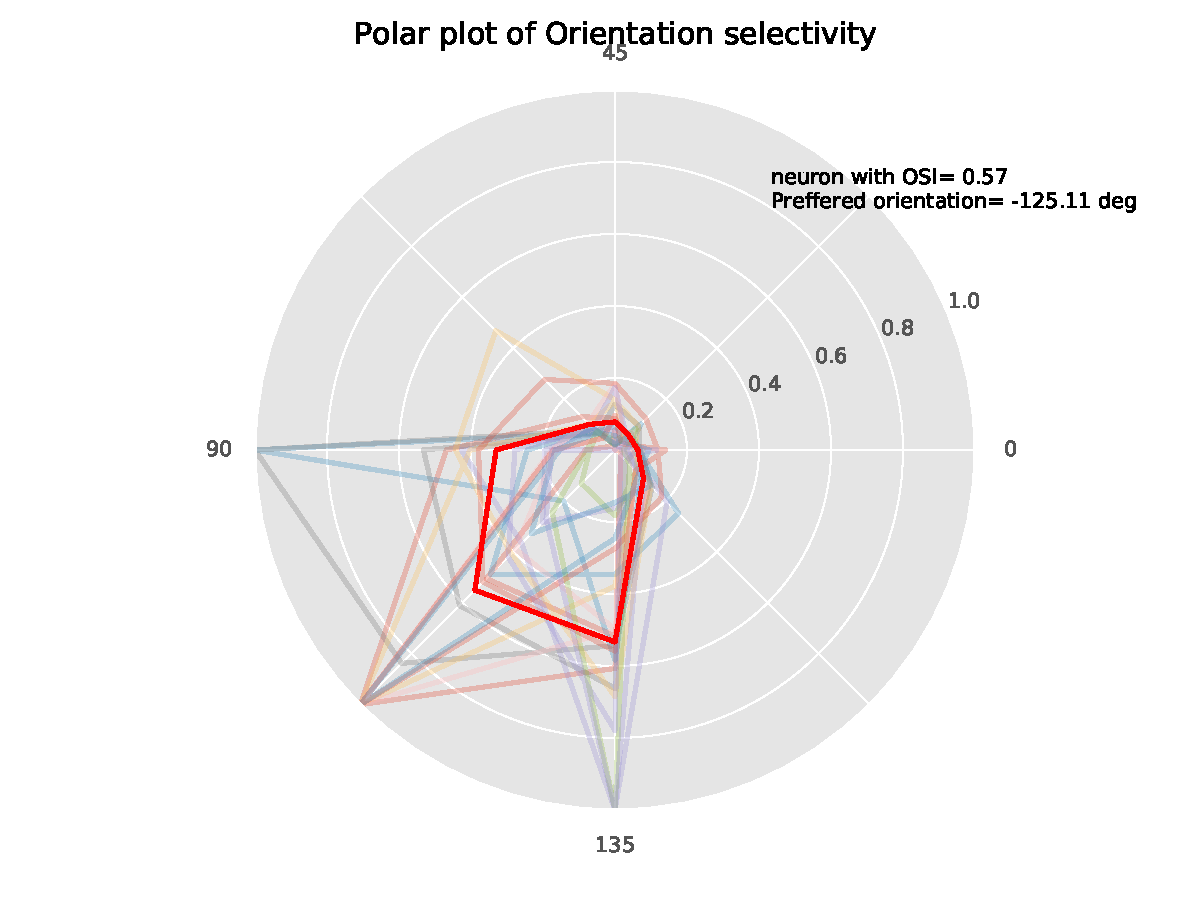
\includegraphics[width=\linewidth]{\plt/gratings_oripolar_2016_04_24_14_08_33.pdf}
    \caption{Responses plotted in orientation space}
    \label{fig:ori_simple}
  \end{subfigure}%
  \begin{subfigure}[b]{0.5\textwidth}
    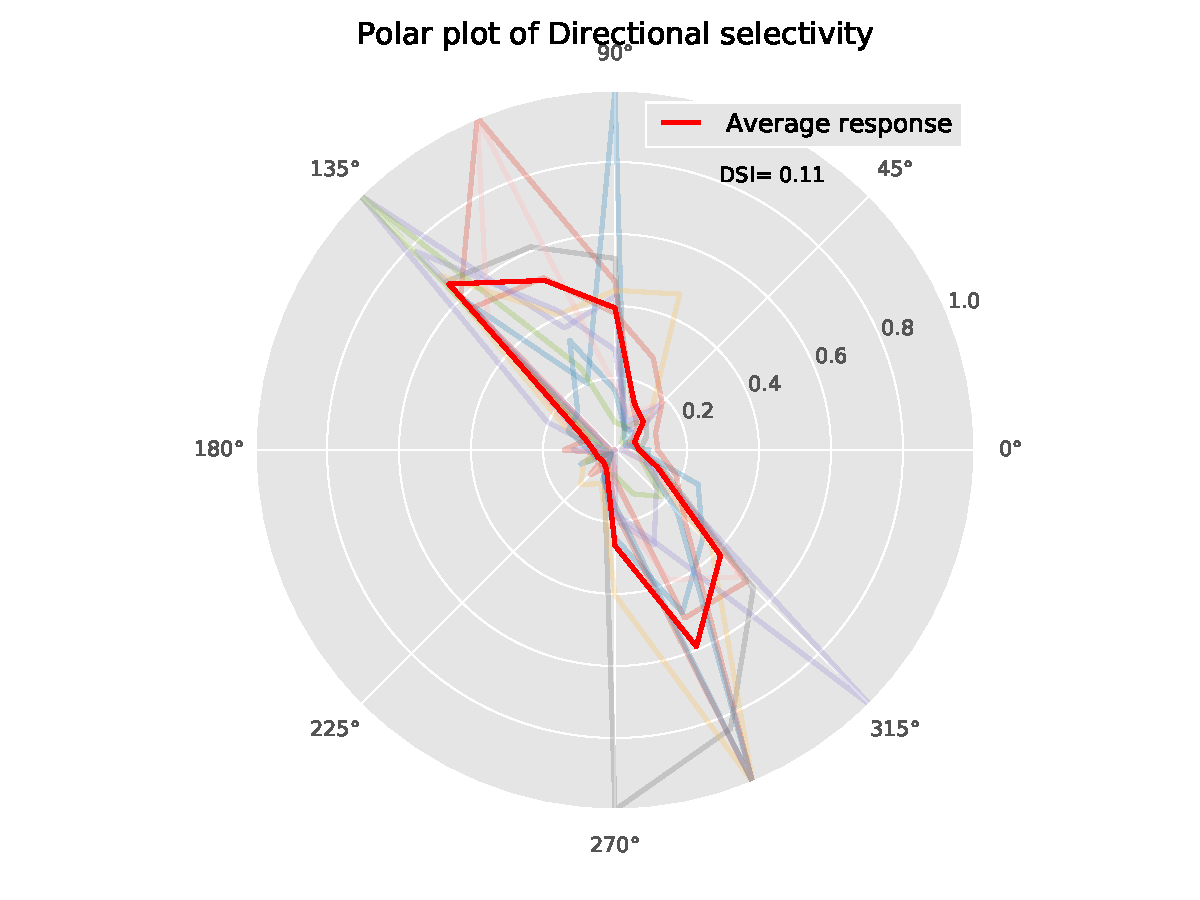
\includegraphics[width=\linewidth]{\plt/gratings_dirpolar_2016_04_24_14_08_33.pdf}
    \caption{Responses plotted in direction space}
    \label{fig:dir_simple}
  \end{subfigure}%
  \caption{Responses $R(\theta_k)$ of a simple neuron for each $\theta_k$ plotted in both orientation and direction space. Equal lobes in direction space shows direction is irrelevant.}\label{fig:oridir_simple}
\end{figure}

A complex neuron is expected to have high OSI and high DSI. Polar plots of responses in orientation and direction space is shown in Figure~\ref{fig:oridir_complex}
\begin{figure}[h]
  \begin{subfigure}[b]{0.5\textwidth}
    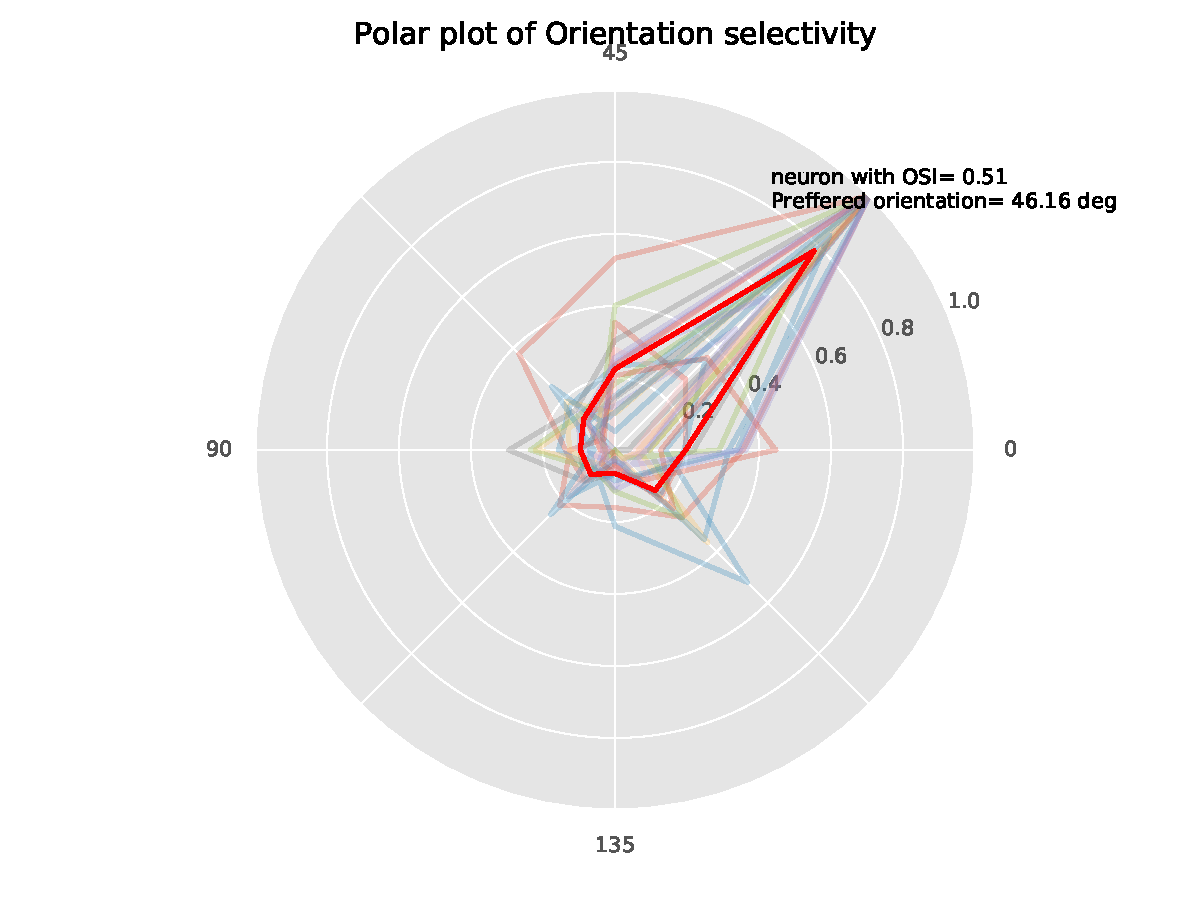
\includegraphics[width=\linewidth]{\plt/gratings_oripolar_2016_05_01_15_25_00.pdf}
    \caption{Responses plotted in orientation space}
    \label{fig:ori_complex}
  \end{subfigure}%
  \begin{subfigure}[b]{0.5\textwidth}
    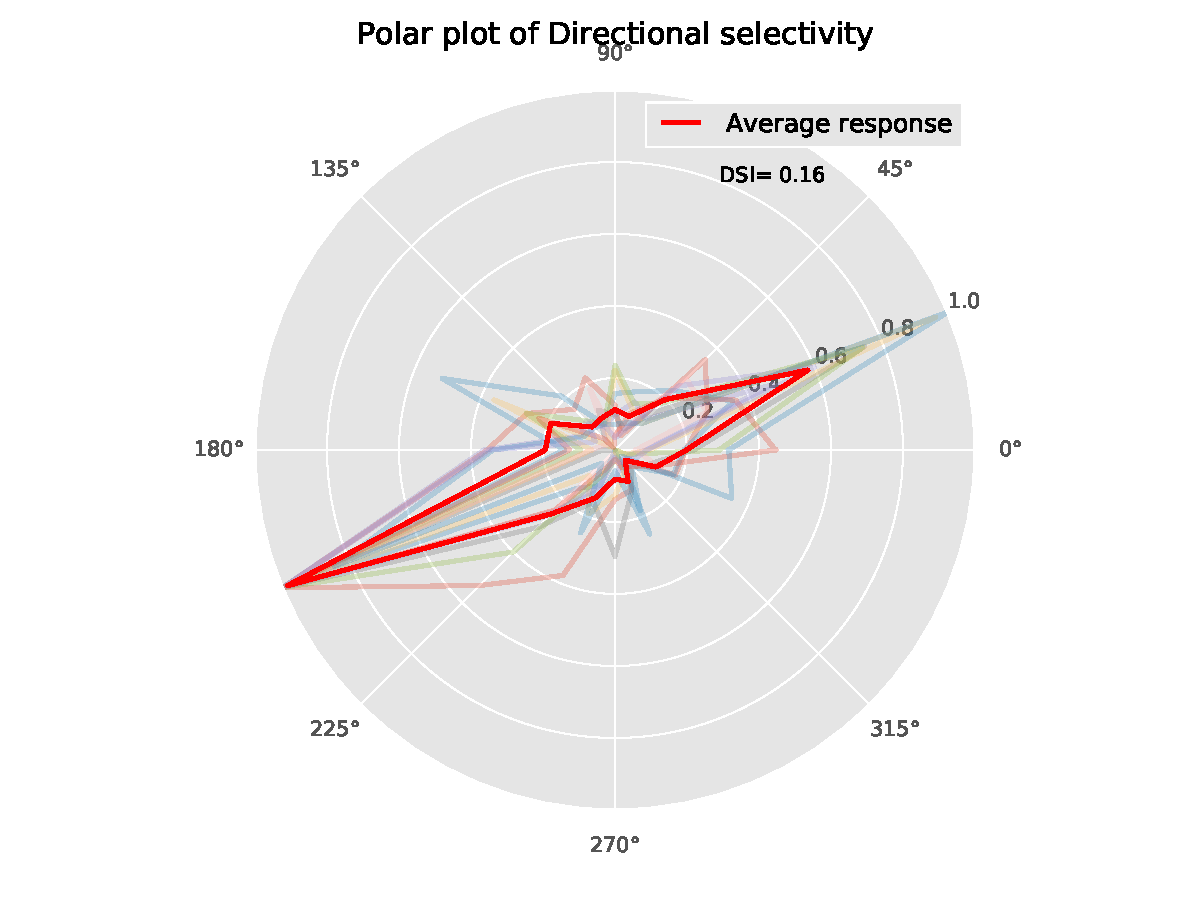
\includegraphics[width=\linewidth]{\plt/gratings_dirpolar_2016_05_01_15_25_00.pdf}
    \caption{Responses plotted in direction space}
    \label{fig:dir_complex}
  \end{subfigure}%
  \caption{Responses $R(\theta_k)$ of a complex neuron for each $\theta_k$ plotted in both orientation and direction space. Unequal lobes in direction space shows one direction is preferred than its opposite.}\label{fig:oridir_complex}
\end{figure}

An orientation insensitive neuron is expected to have low values for both OSI and DSI. Polar plots of responses in orientation and direction space is shown in Figure~\ref{fig:oridir_unsel}.
\begin{figure}[h]
  \begin{subfigure}[b]{0.5\textwidth}
    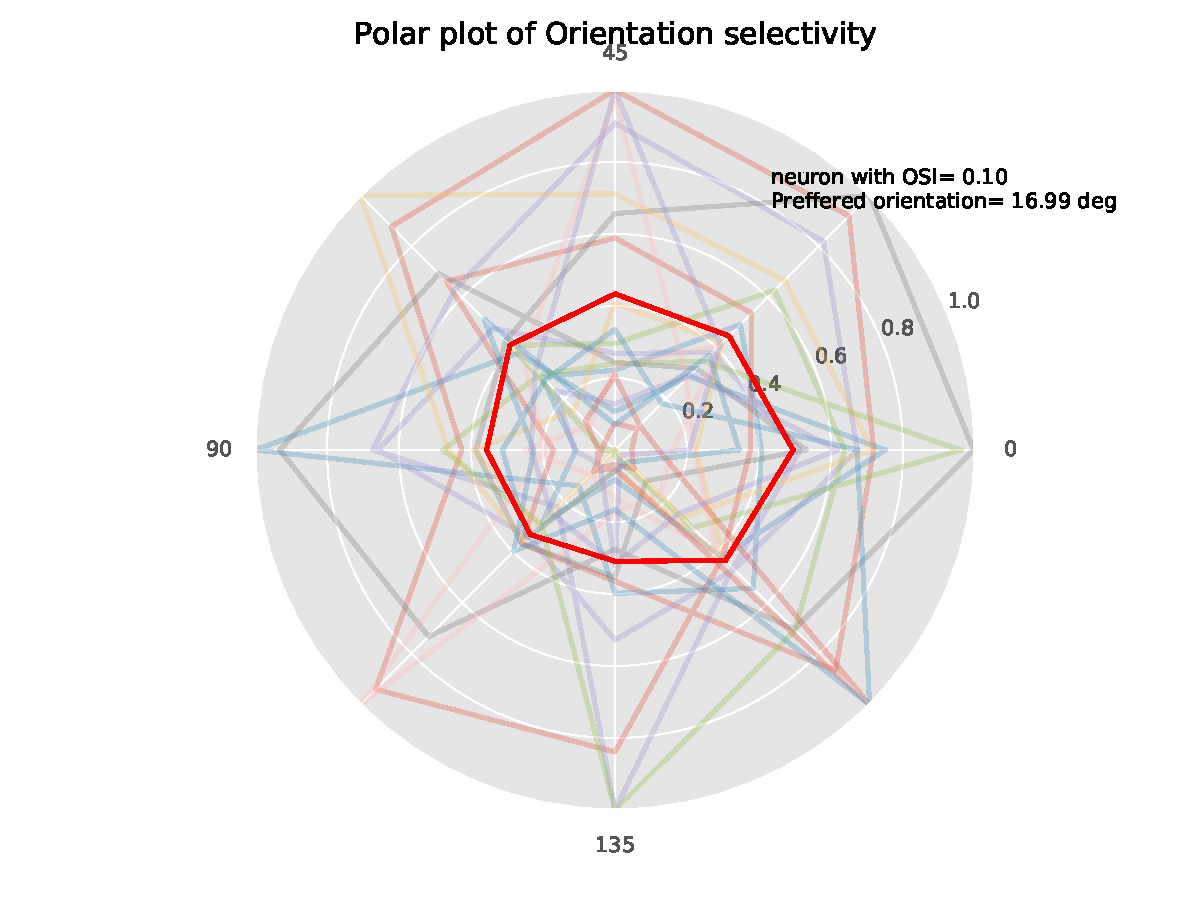
\includegraphics[width=\linewidth]{\plt/gratings_oripolar_2016_05_01_15_26_41.pdf}
    \caption{Responses plotted in orientation space}
    \label{fig:ori_unsel}
  \end{subfigure}%
  \begin{subfigure}[b]{0.5\textwidth}
    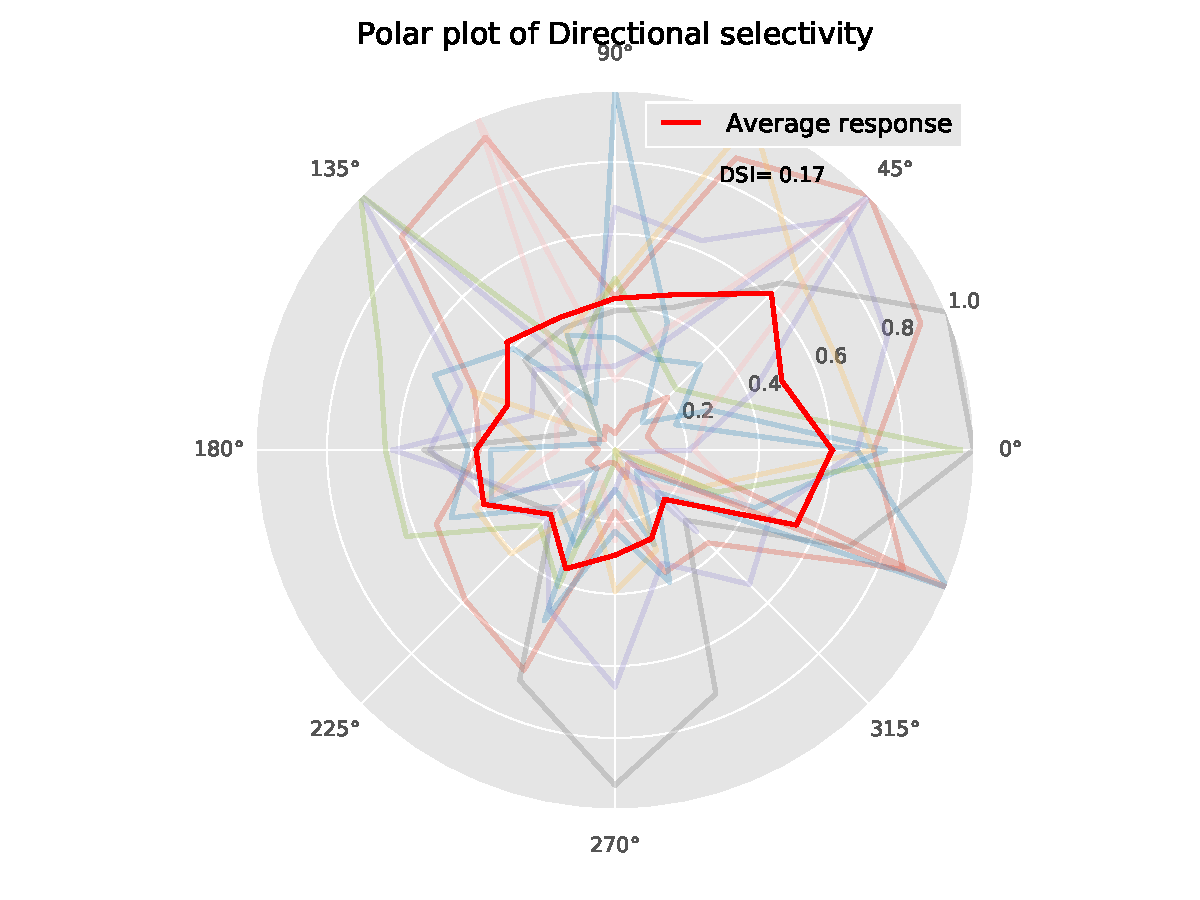
\includegraphics[width=\linewidth]{\plt/gratings_dirpolar_2016_05_01_15_26_41.pdf}
    \caption{Responses plotted in direction space}
    \label{fig:dir_unsel}
  \end{subfigure}%
  \caption{Responses $R(\theta_k)$ of a an orientation insensitive neuron for each $\theta_k$ plotted in both orientation and direction space. Similar responses to all orientations shows absence of selectivity.}\label{fig:oridir_unsel}
\end{figure}
% section quantifying_orientation_and_directional_selectivity (end)

\section{Modeling neuronal response} % (fold)
\label{sec:modeling_neuronal_response_to_sinusoidal_gratings_stimuli}
Modeling the response of neuron to various orientations and visualizing is a great way to see if in fact there is an orientation selectivity. If the cell seems selective, we can also characterize the degree of selectivity and preferred orientation from model parameters.

Orientation tuning curve is modeled using a Gaussian function with constant offset. The empirical form of the orientation tuning curve is,
$$R_o(\theta) = C + R_p \exp\left\{\frac{-||\theta-\theta_{pref}||^2}{2\sigma^2}\right\}$$
Where $R_o(\theta)$ is the time-averaged response of neuron to angle of orientation $\theta$. Parameter $\theta_{pref}$ is the preferred orientation of the neuron. Tuning width $\sigma$  tell us how much the cell is selective. $C$ is a constant offset.

Similarly, we can model direction tuning curve using a mixture of Gaussian functions with a constant offset. 
$$R_d(\theta) = C + R_p \exp\left\{\frac{-||\theta-\theta_{pref}||^2}{2\sigma_1^2}\right\} + R_n \exp\left\{\frac{-||\theta-\theta_{null}||^2}{2\sigma_2^2}\right\}$$
Where $R_o(\theta)$ is the time-averaged response of neuron to angle of direction $\theta$. Relative magnitude of tuning widths, $\sigma_1$ and $\sigma_2$ denote the amount of directional selectivity. $C$ is a constant offset.
% section modeling_neuronal_response_to_sinusoidal_gratings_stimuli (end)

Parameters are estimated by minimizing squared sum of error. Sum of squared error is defined as:
$$SSE = \sum_{i=1}^N ||R(\theta_i) - R_o(\theta_i)||^2$$
A gradient descent algorithm finds the optimum parameters by minimizing SSE.
In Figure~\ref{fig:curvefit_complex} , fit of tuning curves of a complex cell is given. The distinct peak in the orientation tuning curve shows selectivity to orientation $\theta_{pref}$. In the direction tuning curve, peaks of different magnitude shows one direction is more preferred than other.
\begin{figure}[h]
  \begin{subfigure}[b]{0.5\textwidth}
    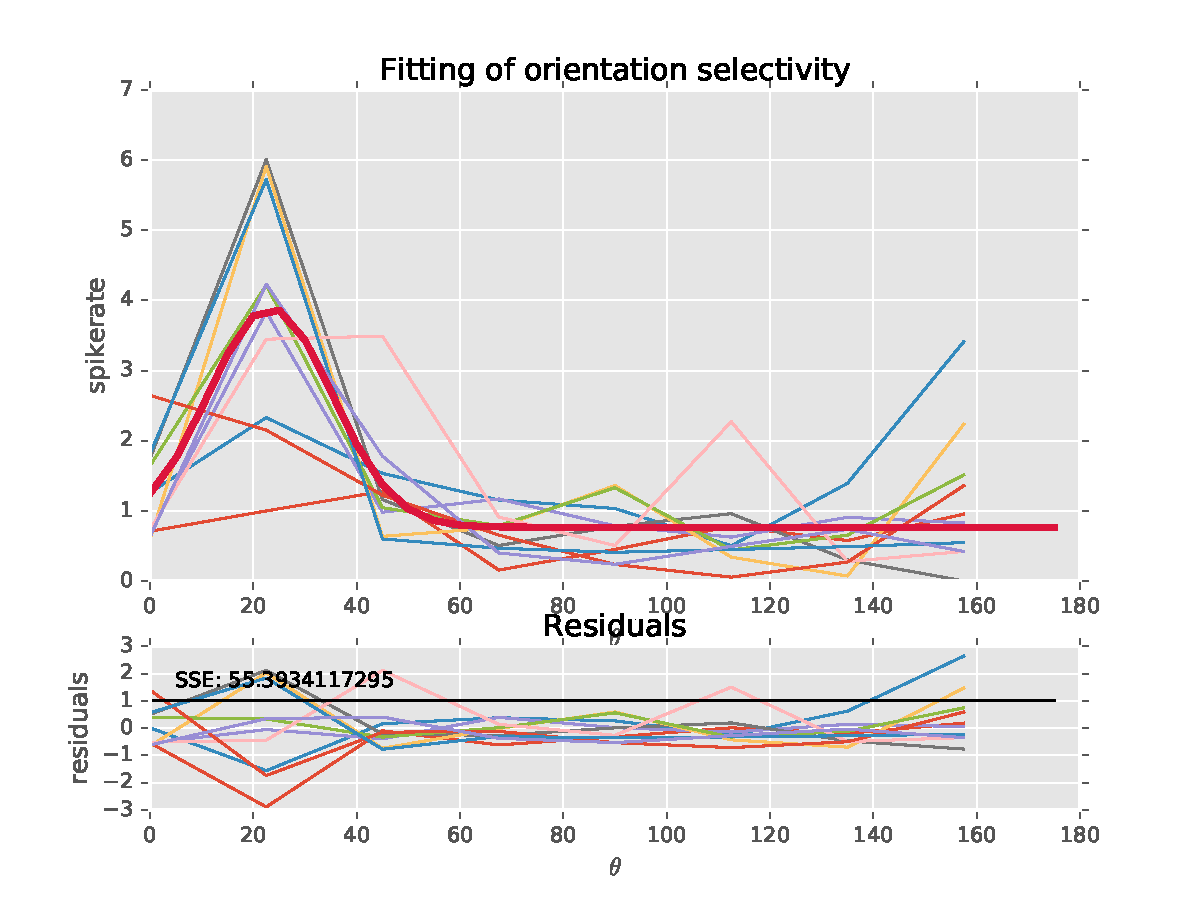
\includegraphics[width=\linewidth]{\plt/gratings_crvefit_osi_n_3_2016_05_02_12_53_03.pdf}
    \caption{Orientation tuning curve}
    \label{fig:oritune_complex}
  \end{subfigure}%
  \begin{subfigure}[b]{0.5\textwidth}
    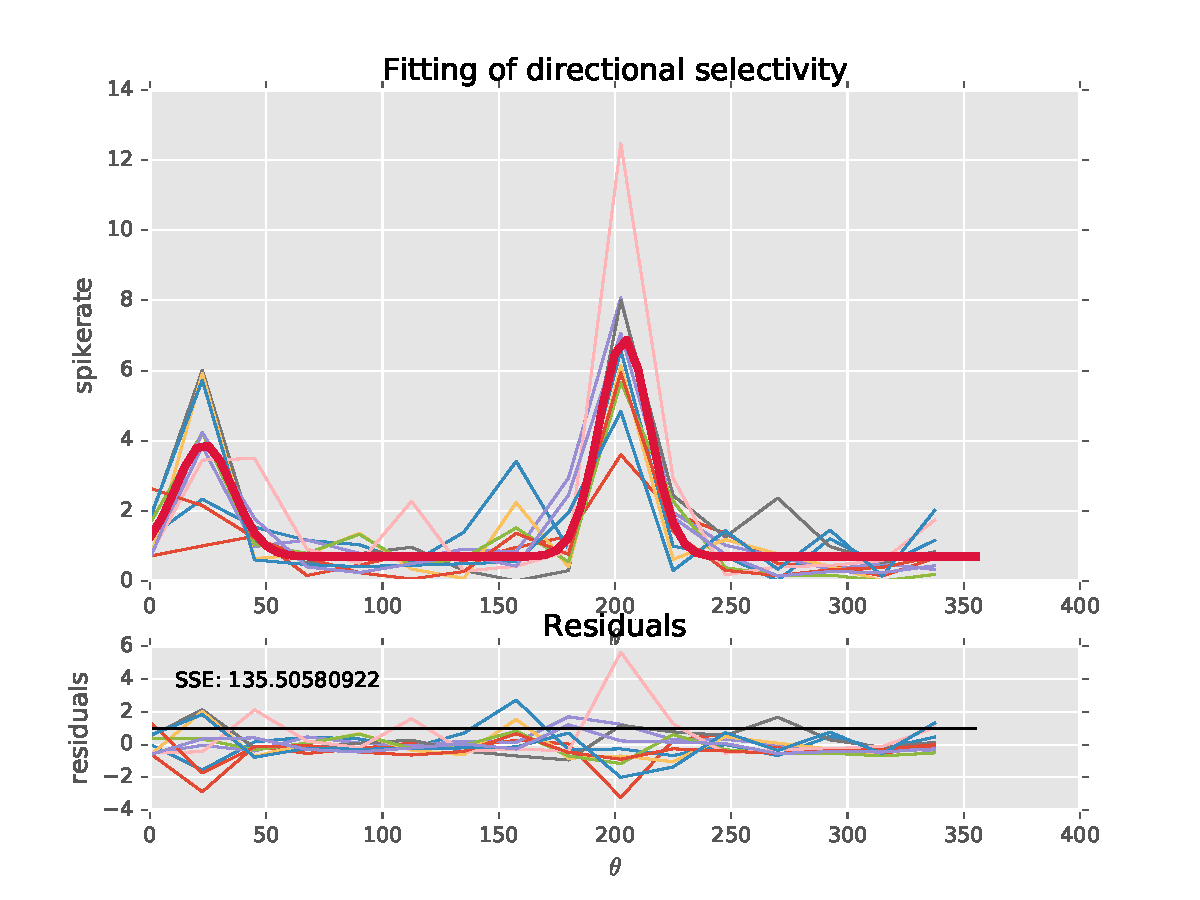
\includegraphics[width=\linewidth]{\plt/gratings_crvefit_n_3_2016_05_01_15_40_28.pdf}
    \caption{Direction tuning curve}
    \label{fig:dirtune_complex}
  \end{subfigure}%
  \caption{Fit of orientation and direction tuning curves of a neuron. The distinct peak in the orientation tuning curve shows selectivity to orientation $\theta_{pref}$. Different $\sigma_1$ and $\sigma_2$ in direction tuning curve shows direction sensitive cell. - Thus a complex cell}\label{fig:curvefit_complex}
\end{figure}
In Figure~\ref{fig:curvefit_simple} , fit of tuning curves of a complex cell is given. The distinct peak in the orientation tuning curve shows selectivity to orientation $\theta_{pref}$. In the direction tuning curve, peaks of same magnitude shows of stimuli direction is irrelevant.
\begin{figure}[h]
  \begin{subfigure}[b]{0.5\textwidth}
    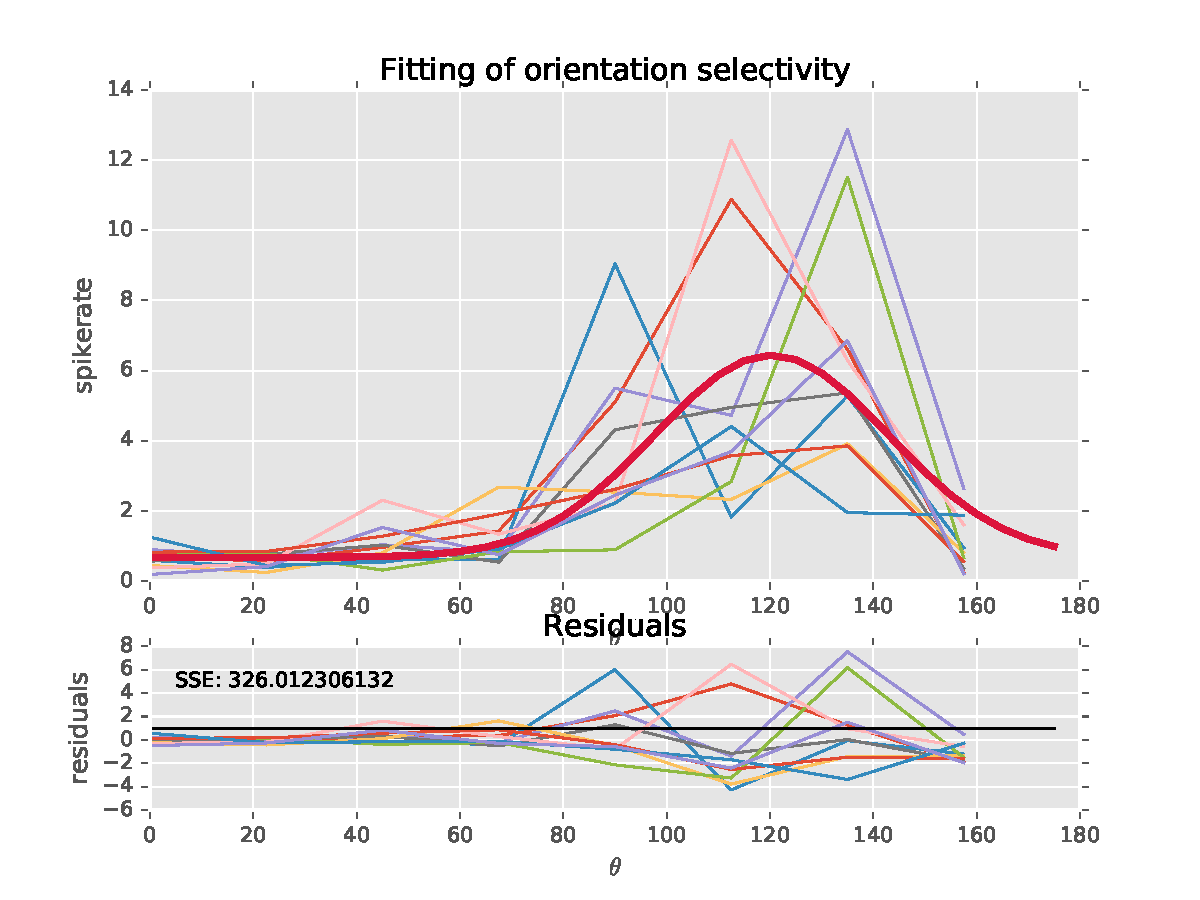
\includegraphics[width=\linewidth]{\plt/gratings_crvefit_osi_n_0_2016_05_02_12_52_43.pdf}
    \caption{Orientation tuning curve}
    \label{fig:oritune_simple}
  \end{subfigure}%
  \begin{subfigure}[b]{0.5\textwidth}
    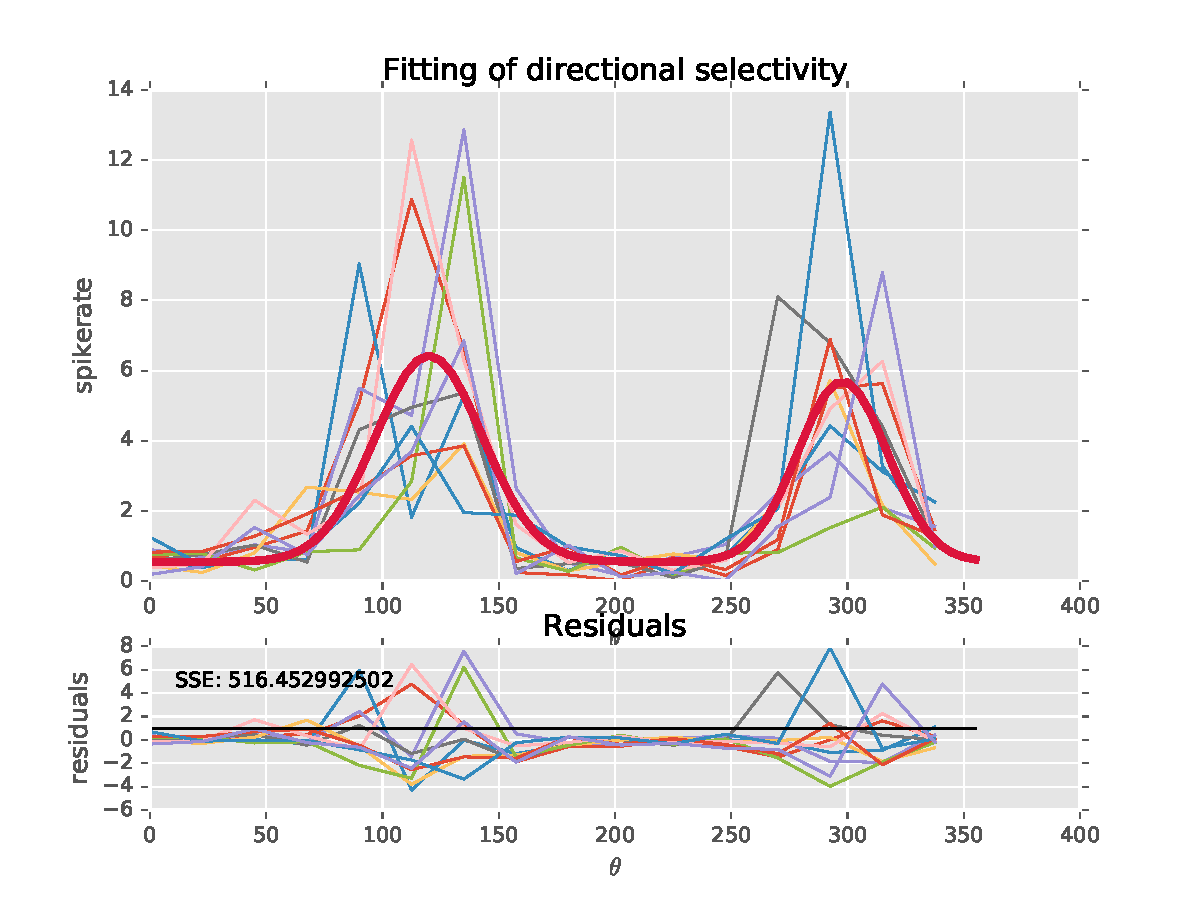
\includegraphics[width=\linewidth]{\plt/gratings_crvefit_n_0_2016_05_01_15_40_26.pdf}
    \caption{Direction tuning curve}
    \label{fig:dirtune_simple}
  \end{subfigure}%
  \caption{Fit of orientation and direction tuning curves of a neuron. The distinct peak in the orientation tuning curve shows selectivity to orientation $\theta_{pref}$. Similar $\sigma_1$ and $\sigma_2$ in direction tuning curve direction of stimuli is irrelevant. - Thus a simple cell}\label{fig:curvefit_simple}
\end{figure}
\section{Finding similarly tuned neurons} % (fold)
\label{sec:finding_similarly_tuned_neurons}
Receptive field of a neuron in V1 consists of a subset of neurons in one layer below it. Those neurons in turn have a receptive field. By following layers down, we can find a visual field for each neuron in V1. Orientation selectivity of neurons in V1 detects edges and their orientation in images. By studying similarly tuned neurons, we can get an insight to redundancy of coding and distribution of functionally similar cells in V1.

Similarly tuned cells are expected to have similar response to different stimuli orientations. A high correlation of responses $R(\theta_k)$ to various angle $\theta_k$ will represent similarly tuned cells. Even after having same preferred orientations, the neurons could have different degree of selectivity. We would like to find similarly tuned neurons which have an `acceptable' OSI.

Pearson correlation between each pair of neurons in a mice are computed and plotted in Figure~\ref{fig:corr}. The neurons in both axes have a decreasing OSI value. The neuron pairs that lei in bottom left of the Figure~\ref{fig:corr} are the ones we have interested. Finally to find neurons that are similarly tuned to a particular neuron, choose the corresponding row and all the neurons in that row having good correlation value and having acceptable OSI are selected. Figure~\ref{fig:tunecurves} shows tuning curves of some neurons retrieved from correlation study.
\begin{figure}[h]
  \centering
  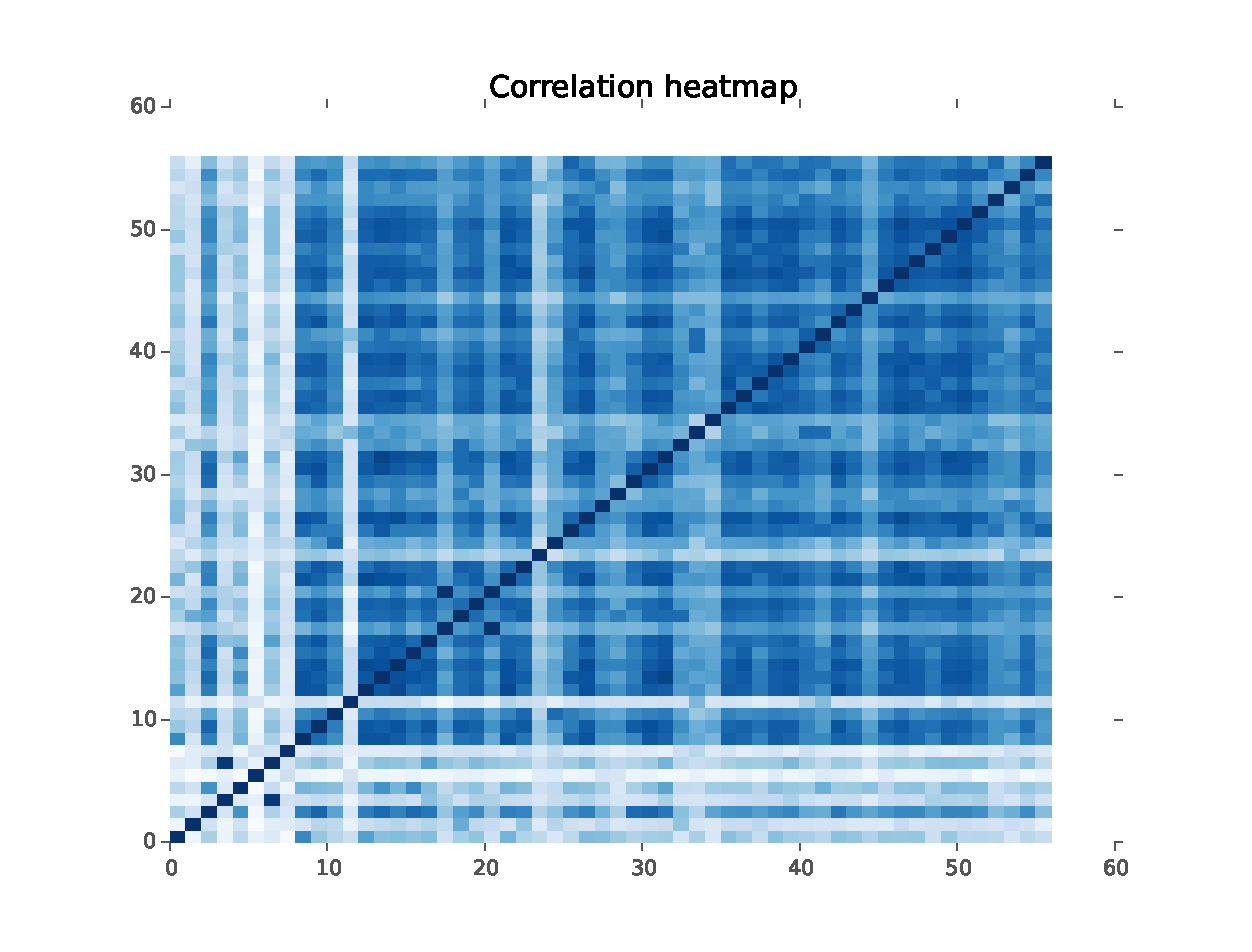
\includegraphics[width=.9\linewidth]{\plt/tuningCorr_desc_civar_m2}
  \caption{Pairwise Pearson correlation of neurons. Both axes are sorted in decreasing order of OSI.}
  \label{fig:corr}
\end{figure}
\begin{figure}[h]
  \centering
  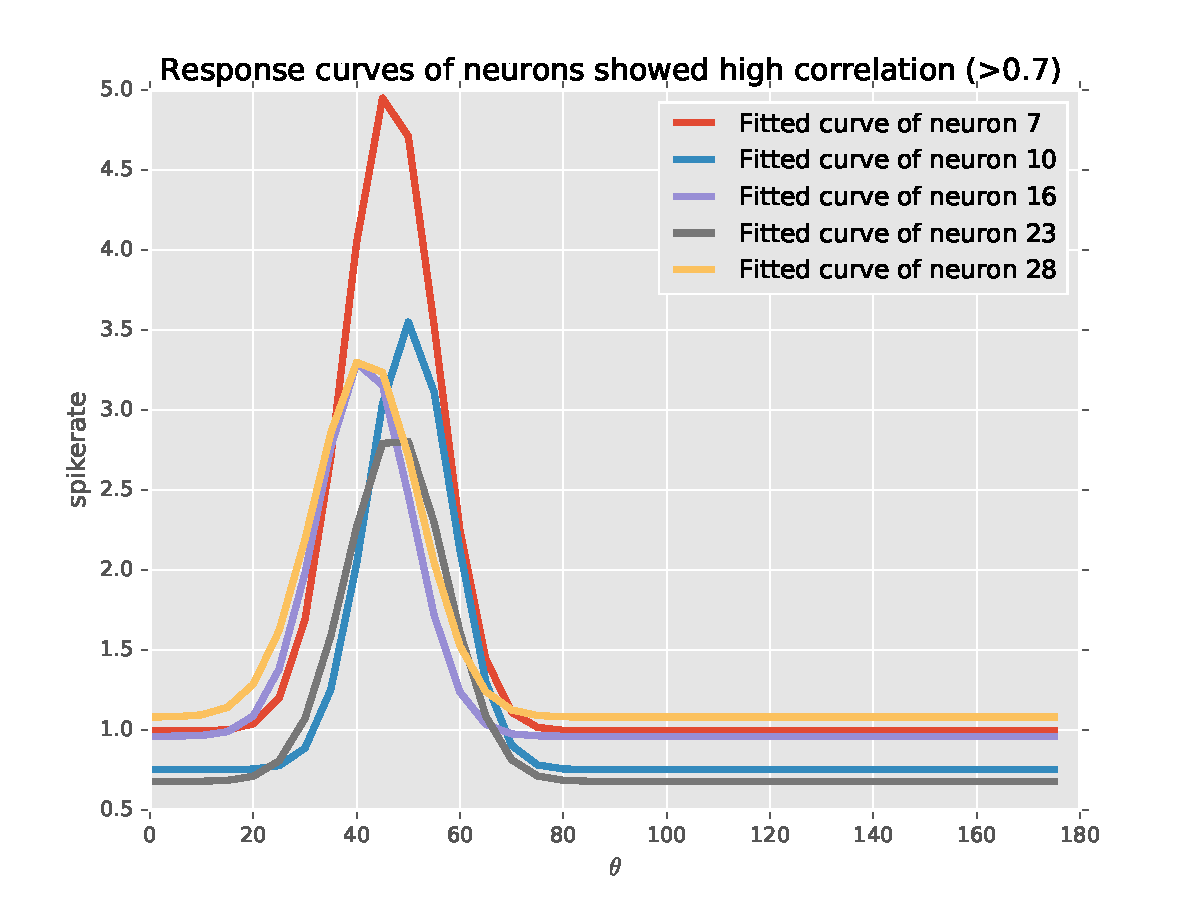
\includegraphics[width=.9\linewidth]{\plt/gratings_sel_model_2016_05_02_15_57_20.pdf}
  \caption{Orientation tuning curves of some neurons retrieved from correlation study. All of them have a same preferred orientation.}
  \label{fig:tunecurves}
\end{figure}

\section{Study of principal components} % (fold)
\label{sec:study_of_correlation}
Information contained in the visual stimuli reaches V1 after it gets passed through lower layers. Edges and motion of edges in the stimuli are represented by orientation and direction sensitive neurons in V1. Through Principal Component Analysis (PCA) we aim to study the tightness of information representation. A subset of neurons ($\sim 60$) in V1 are sampled at 20Hz for 6 seconds during the experiment. We analyze principal components of the responses to find redundancy in the responses. The number of uncorrelated principal components which capture `most' of the variance in data can determine redundancy.

Principal Component Analysis is an orthogonal transformation of possibly correlated observations to linearly uncorrelated components called principal components.  The principal components are orthogonal because they are the eigenvectors of the covariance matrix, which is symmetric. The first principal component captures largest variance and decreases further. By observing number of components that needs to capture a desired variance, we can tell correlations in the data. Transforming original data to new orthogonal basis gives a representation which has dimension less than or equal to the number of original dimension. Reconstructing original data from subset of principal components also indicates amount of correlation in original data.

Here we take number of neurons as feature dimension. The responses are averages across trials.  PCA is done on the data to find ratio between number of principal components and variance explained. Figure~\ref{img:pca} shows the result for a mouse towards a sinusoidal grating stimuli. The original data was transformed to principal components basis with a subset of principal components. Attempting to reconstructing original data from transformed data produces an error. The reconstruction error depends on number of chosen subset of principal components. Figure shows reconstruction error for different number of principal components. As we increase number of principal components, the error decreases. And finally as the number components equals the original feature dimension, reconstruction error vanish.

\begin{figure}
    \centering
    \begin{subfigure}[b]{.48\textwidth}
        \centering
        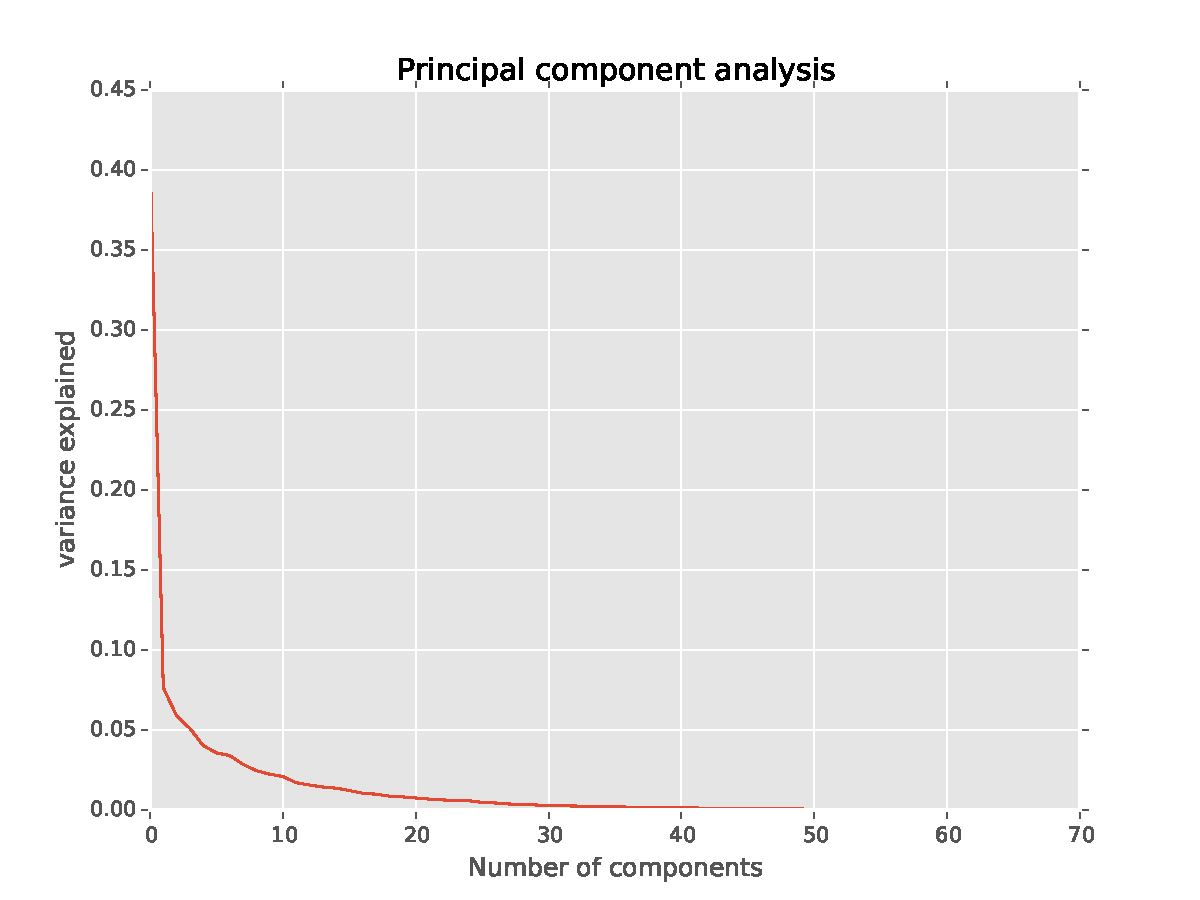
\includegraphics[width=\linewidth]{\plt/subsetbMain_pcaPlot_2016_02_05_15_41_05.pdf}
        \caption{Variance captured by components}
        \label{img:pca}
    \end{subfigure}
    ~
    \begin{subfigure}[b]{.48\textwidth}
        \centering
        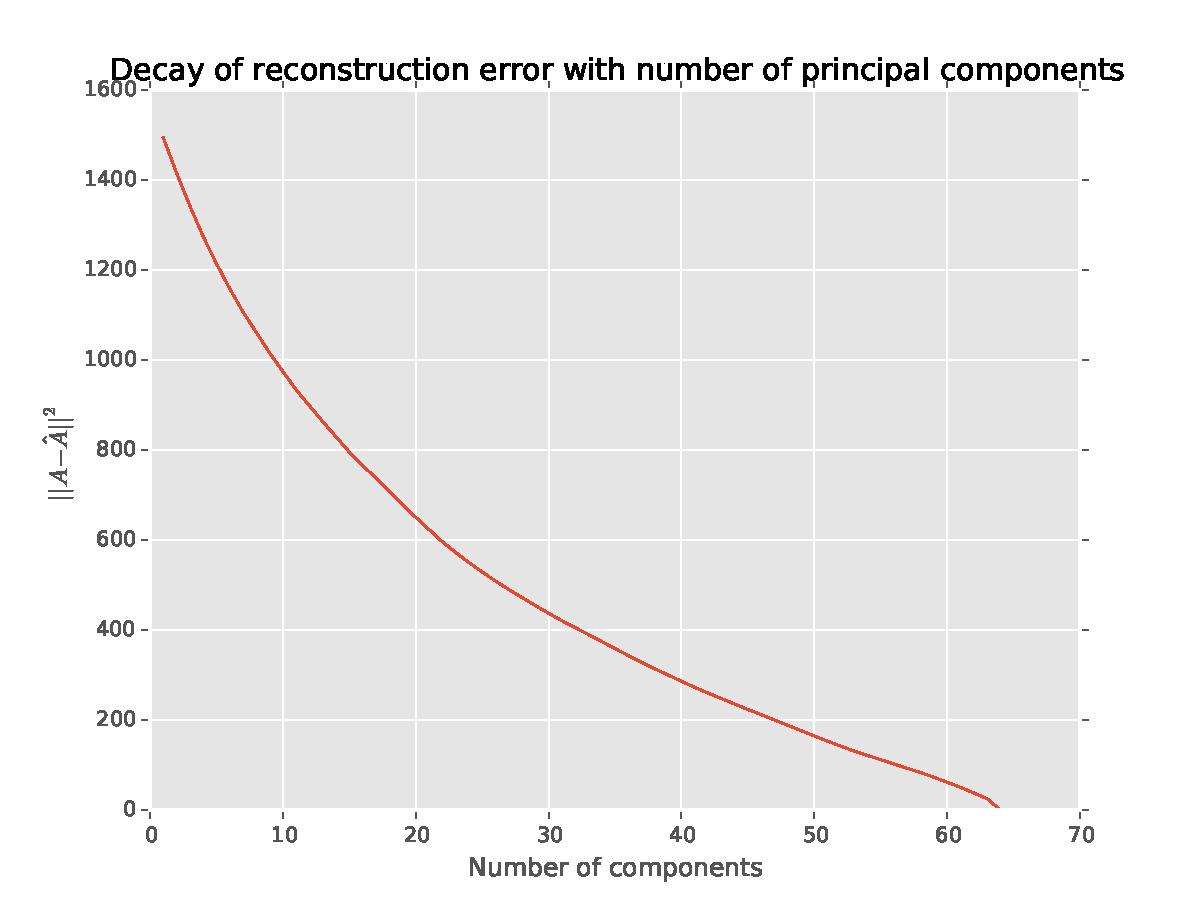
\includegraphics[width=\linewidth]{\plt/subsetbMain_errPlot_2016_02_12_12_42_39.pdf}
        \caption{Decay of reconstruction error}
        \label{img:reconstruction}
    \end{subfigure}
    \caption{Principal Component Analysis of response of neuron to drifting sinusoidal grating stimuli.}
\end{figure}

\section{Study of Reliability} % (fold)
\label{sec:study_of_reliability}
Information encoding in primary visual cortex is a complex process due to intrinsic neuronal variability. Intertrial reliability of information encoding in neurons is the first step into analyzing coding mechanism of V1. The degree of trial-to-trial variability in a response is com-
monly measured in terms of reliability. A neuron is said to be reliable if it fires the same number of precisely timed spikes on every repetition of a stimulus [\cite{tiesinga2008regulation}].

The experiment performed measures calcium concentration in neurons rather than spike rate. Trial to trial reliability can be computed using correlation between responses of each trial. When a visual stimuli is presented $T$ times, we can compute response reliability $R_A$ of a neuron to the stimuli $A$.
$$R_A = \frac{2}{T^2 - T}\sum_{i=1}^T \sum_{j=i+1}^T \rho(f_{i, A}, f_{j, A})$$
where $f_{i, A}$ is the response of neuron to $i^{th}$ trial of movie A and $\rho$ is the Pearson correlation.

The study was done for 48 neurons in a mice and the response reliability is plotted in Figure~\ref{img:ra} for each neuron. It is evident that response reliability for most of neurons are small. The study shows responses of neurons in V1 are not robust because of intrinsic noise. If the whole sequences is not reliable, could there be subsequences that are reliable? We will explore it in coming chapters by detecting common subsequences.
\begin{figure}
    \centering
    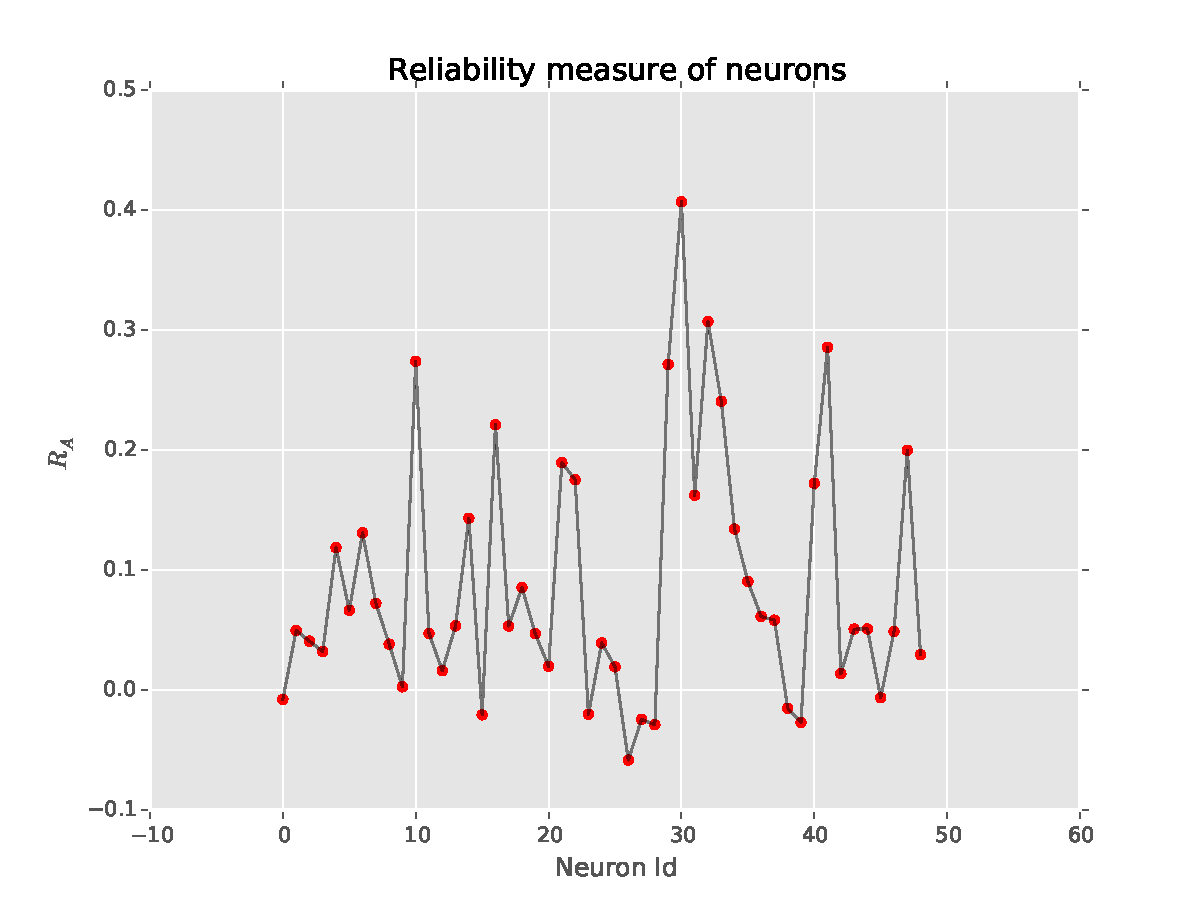
\includegraphics[width=.7\linewidth]{\plt/reliabMain_raPlot_2016_02_05_13_25_56.pdf}
    \caption{Reliability measure $R_A$ for different neurons}
    \label{img:ra}
\end{figure} 
% section study_of_reliability (end)
% section finding_similarly_tuned_neurons (end)
%%%%%%%%%%%%%%%%%%%%%%%%%%%%%%%%%%%%%%%%%%%%%%%%%%%%%%%%%%%%%%%%%%%%%%
\chapter{Searching for Motifs}       % 6 pages
\label{chap:searchmotif}
In Music, motif is a perceivable recurring fragment. They are elementary signatures that repeats to form bigger units. Detecting such motifs in a song tells us more about the song like its melody. In Genetics, motif is a sequence pattern of nucleotides in a longer DNA sequence. From a signal processing perceptive, motifs is a signal segment that recurs in a longer signal. A valid motif should have an `acceptable' length such that it has a significance. Motif analysis is import because in every domain, occurrence of motifs has a meaning to it.

In the experiment, each neuron responses are captured as a time series sampled at 20Hz for 10 seconds. In neuron responses we define a Motif as subsequence of response time series which has the following properties:
\begin{itemize}
   \item Recurs in the same response signal but in a different part \textbf{or}
   \item Recurs in the response of the same neuron to a different trial \textbf{or}
   \item Recurs in the response of another neuron in the same mouse \textbf{or}
   \item Recurs in the response of neuron in a different mouse \textbf{and}
   \item Has a significant length in time.
\end{itemize}
Analyzing motifs in neuronal signals will help us understand reliable information representation. Even if two responses of same trial has a long subsequence but not time synchronized, Study of reliability in Section~\ref{sec:study_of_reliability} will fail as the Pearson correlation coefficient will output a small value. Motivic analysis can detect such subsequences even if they are time shifted.

Study of motifs across two different neurons within a mouse can explain correlation between two neurons. Correlated neurons can represent neuronal interconnections. Correlated and synchronous activity in populations of neurons has been observed in many brain regions and has been shown to play a crucial role in cortical coding, attention, and network dynamics [\cite{rosenbaum2014correlated}]. Studying correlations between neurons is again not effective if their responses are time separated as Pearson correlation will fail. Analyzing motifs across neurons will be a better way to study neuronal correlations.

Motifs found in neurons from two \textit{different} mice will represent similar biological process both the neurons undergoes. As the motifs found cannot be due to interconnections, they are due to same activation mechanism of neurons. In this case, we would expect a small motif compared to motifs found within mouse.

In this chapter, we will analyze the presence of motifs in neuronal signals. The presence of motifs will motivate us to extract the motifs and their significance.
\section{Cross-Correlation Function} % (fold)
\label{sec:correlation_function}
Cross correlation is a measure of similarity between two signals as a function of lag of one signal relative to the other. It is commonly used for searching a short query sequence in a large reference sequence. The function calculates sliding dot product at various lags. For discrete signals, cross correlation is defined as:
$$(f \star g)[n]\ \stackrel{\mathrm{def}}{=} \sum_{m=-\infty}^{\infty} f^*[m]\ g[m+n].$$
Searching for a motif using correlation function  is possible if we already have a subsequence that we suspect as a motif. To visualize correlation function in query search, we will manually select a subsequence and search for its occurrences in a neuronal response signal. For the scope of this chapter, we take a subsequence from the response of a `template neuron' and search for its occurrences in response of a `target neuron'.

Trial averaged responses of template and target neurons are taken, then a subset of former is extracted using parameters frame ending and frame width. This subsequence is compared with target sequence as a function of lag. Figure~\ref{img:cacf} shows Cross-Correlation function between a target neuron response and a manually chosen subsequence from template neuron.
\begin{figure}[h]
    \centering
    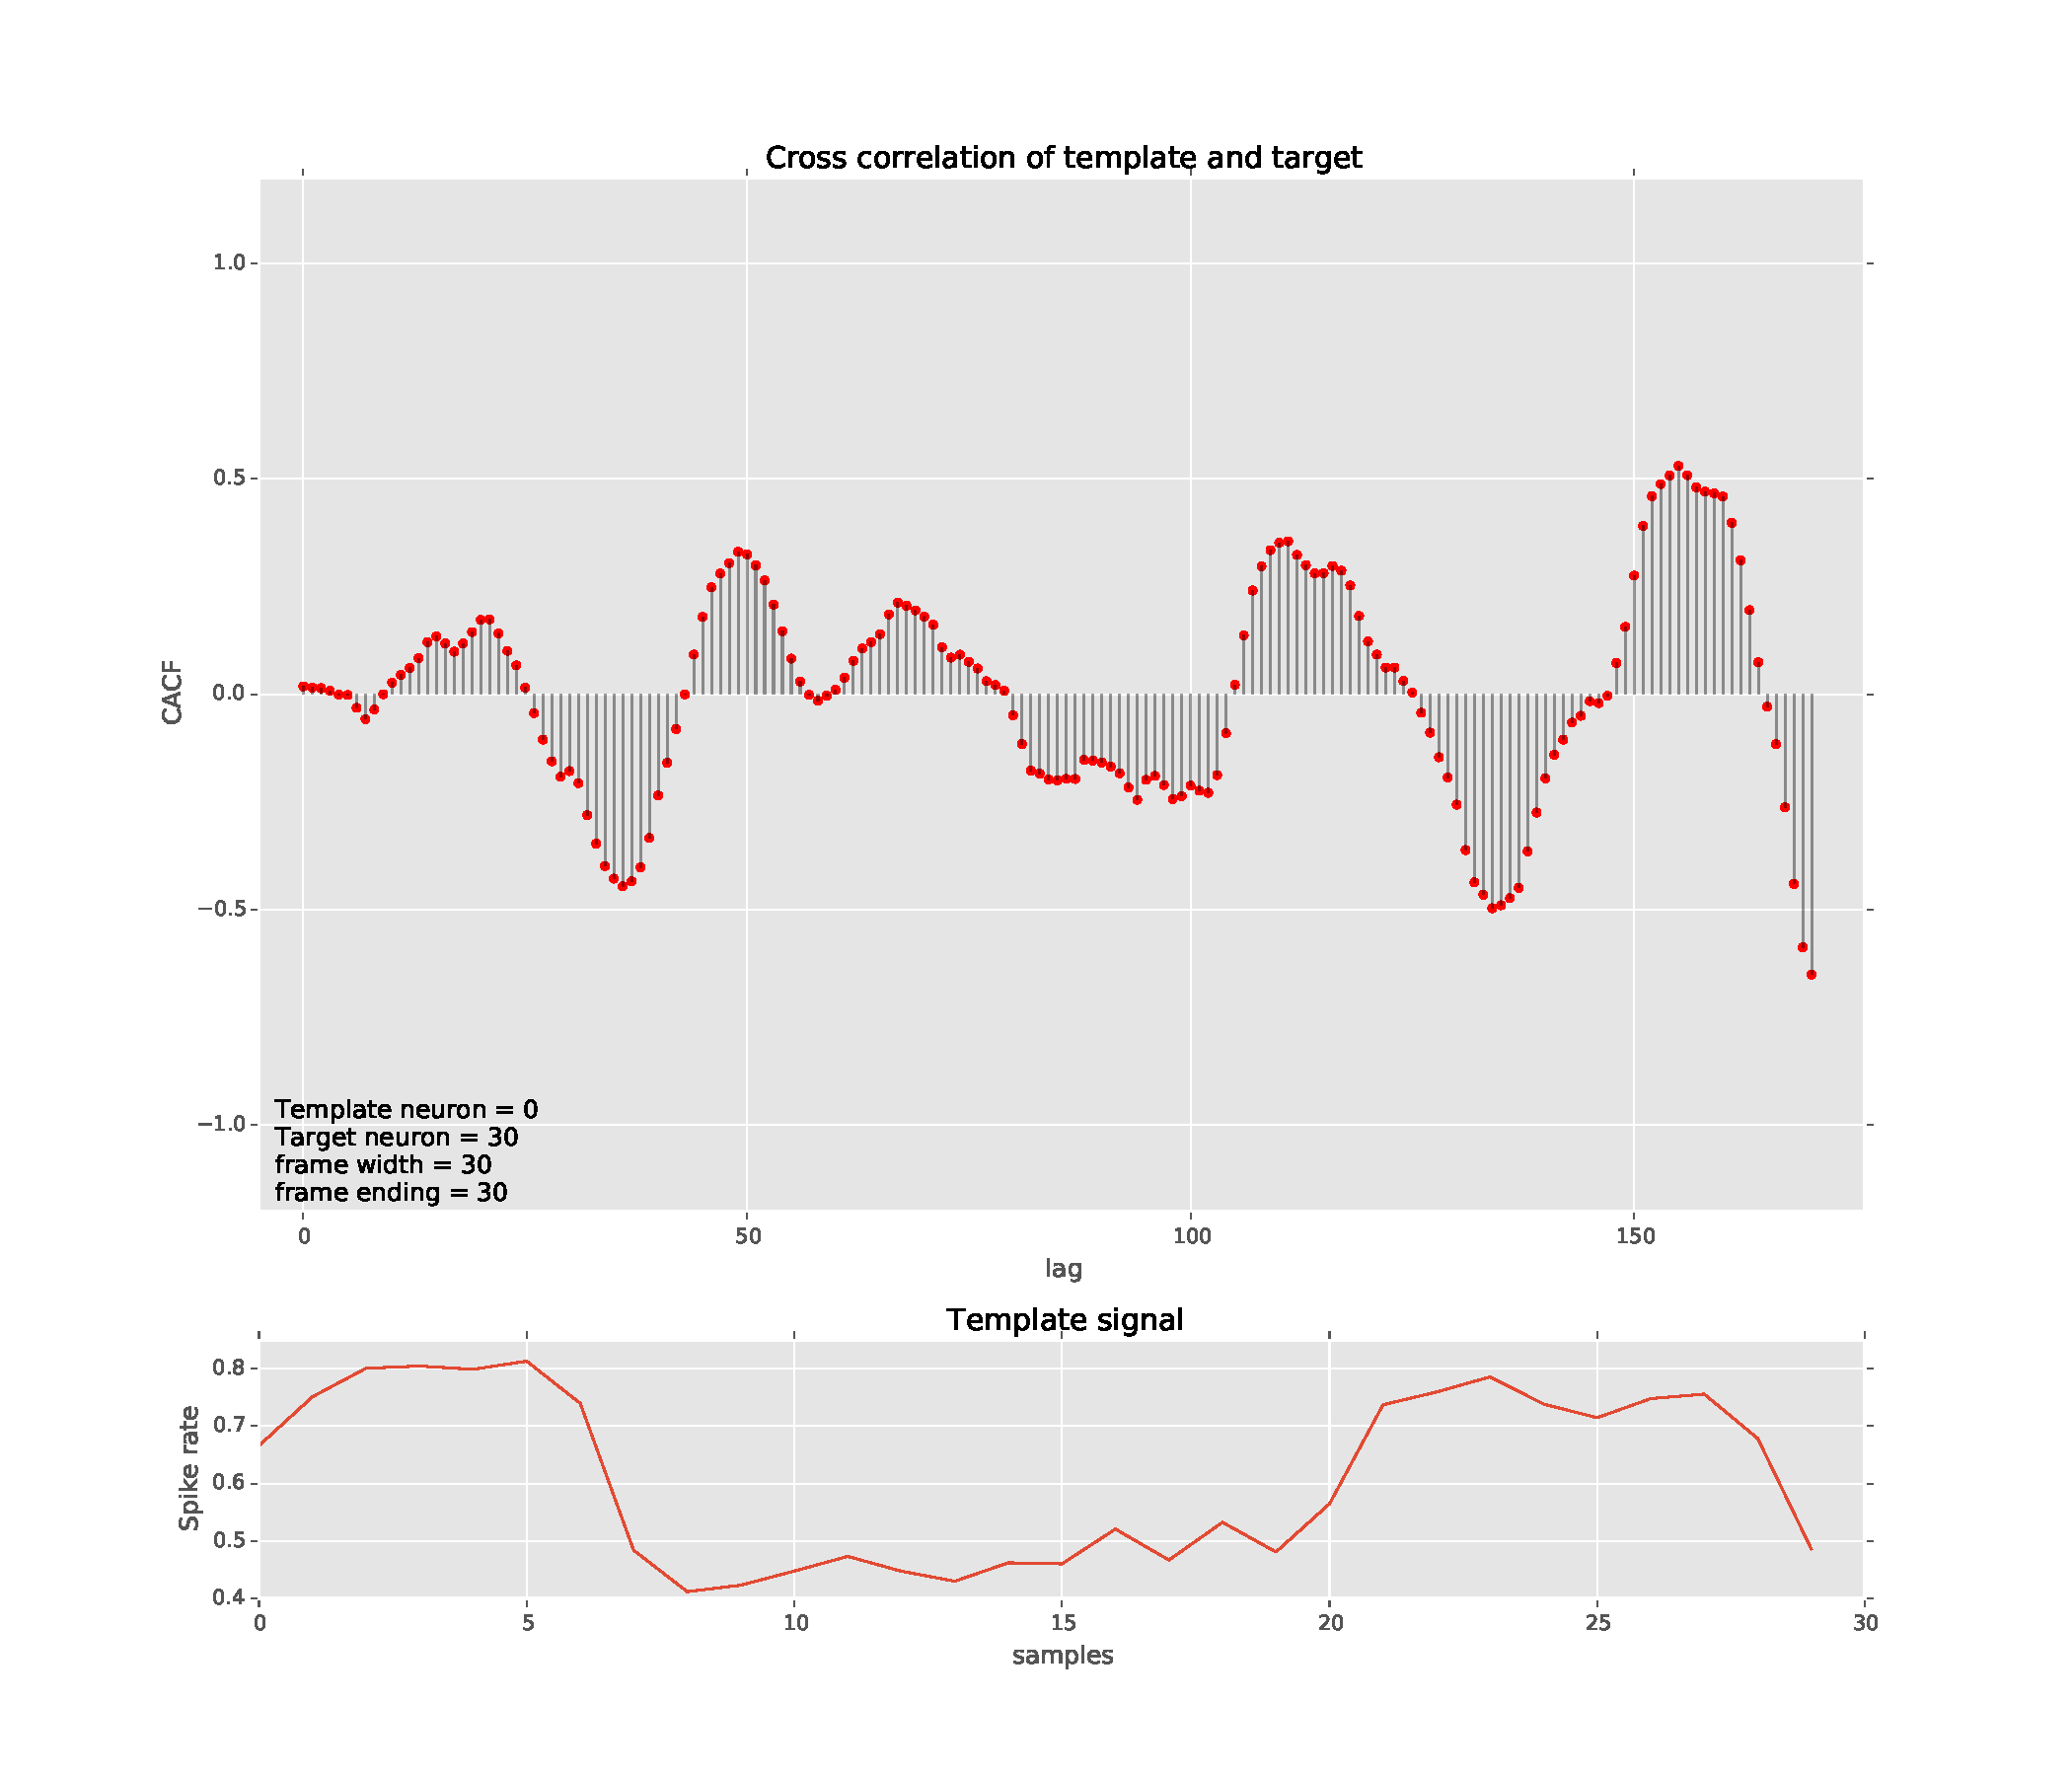
\includegraphics[width=.7\linewidth]{\plt/acfMain_acfPlot_2016_02_05_16_45_37.pdf}
    \caption{Cross-Correlation function between a target neuron response and a manually chosen subsequence from template neuron.}
    \label{img:cacf}
\end{figure}
This study is not effective as we do not know what to search for. Manually selecting a subsequence is inefficient and selected subsequence does not guarantee to be valid motif. 
% section correlation_function (end)
\section{ACFGram} % (fold)
\label{sec:acfgram}
A spectrum describes a signal in terms of energy spread over its frequency components. A spectrogram does exactly the same but also takes  another time into consideration. Computing spectrogram is done by first making chunks/frames of time-domain signal which usually overlap. Magnitude of Fourier transform of each frame is computed to form magnitude spectrum of that frame. These frame spectra are stacked horizontally in increasing order of frame ending time to form a spectrogram. This enables us to study the change of spectra with time.

We formulate an analogous visualization of Cross-Correlation function where the template signal changes in each frame. A frame is a subsequence of original signal with a width and frame ending parameter. Changing the frame ending successively will return overlapping frames having same width. Figure~\ref{img:framesel} shows how a frame from template signal is selected.
\begin{figure}[h]
    \centering
    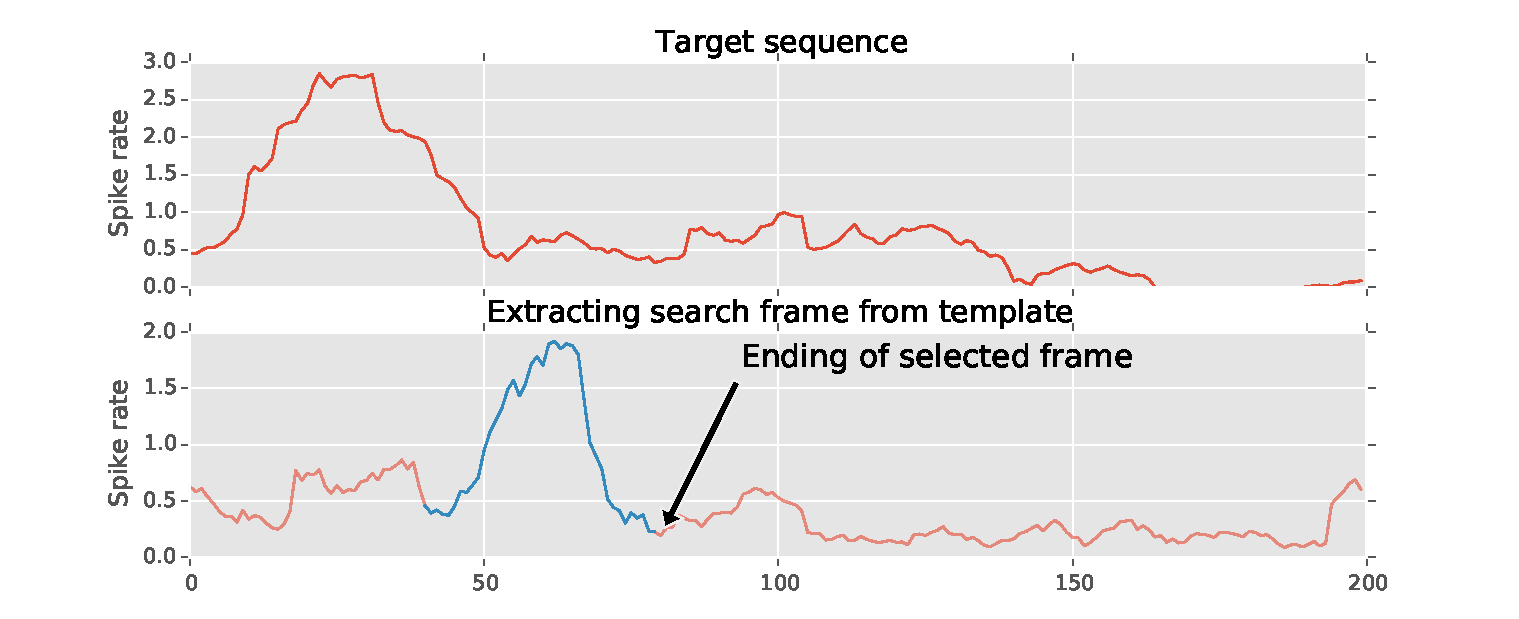
\includegraphics[width=\linewidth]{\plt/framesel.pdf}
    \caption{Extracting frame from template based on frame width and ending.}
    \label{img:framesel}
\end{figure}
Cross-Correlation of extracted frame and target signal at various lags are computed. Next frame is extracted by incrementing frame ending parameter. The process is then repeated for the next frames. Cross-Correlation function of each frame is then stacked horizontally to form a temporal dimension. We call the resulting Time Vs Lag Vs Cross-Correlation function as ACFGram.
% $$ShYaM1193
In the previous study
In Section~\ref{sec:correlation_function} we varied frame width and frame ending manually to extract a signal subsequence and then queried it in target signal. ACFGram removes frame ending parameter. Existence of motifs will be clear if we iterate frame width. The study was conducted across trials of same neuron and across different neurons.

The Figure~\ref{fig:acfgram_same}  shows ACFGram plots for template and target responses from same neuron. The study aim to find presence of repeating subsequence within a neuron's response. The length of suspected motif is varied as a parameter.
For a small frame width ($\sim 15$) the estimation of Cross-Correlation function is poor. Also such a small subsequence is not significant enough to be considered as a motif. As we Increase the frame width, repeating patterns are found which indicates the presence of repeating subsequence.
\begin{figure}[h]
  \begin{subfigure}[b]{0.5\textwidth}
    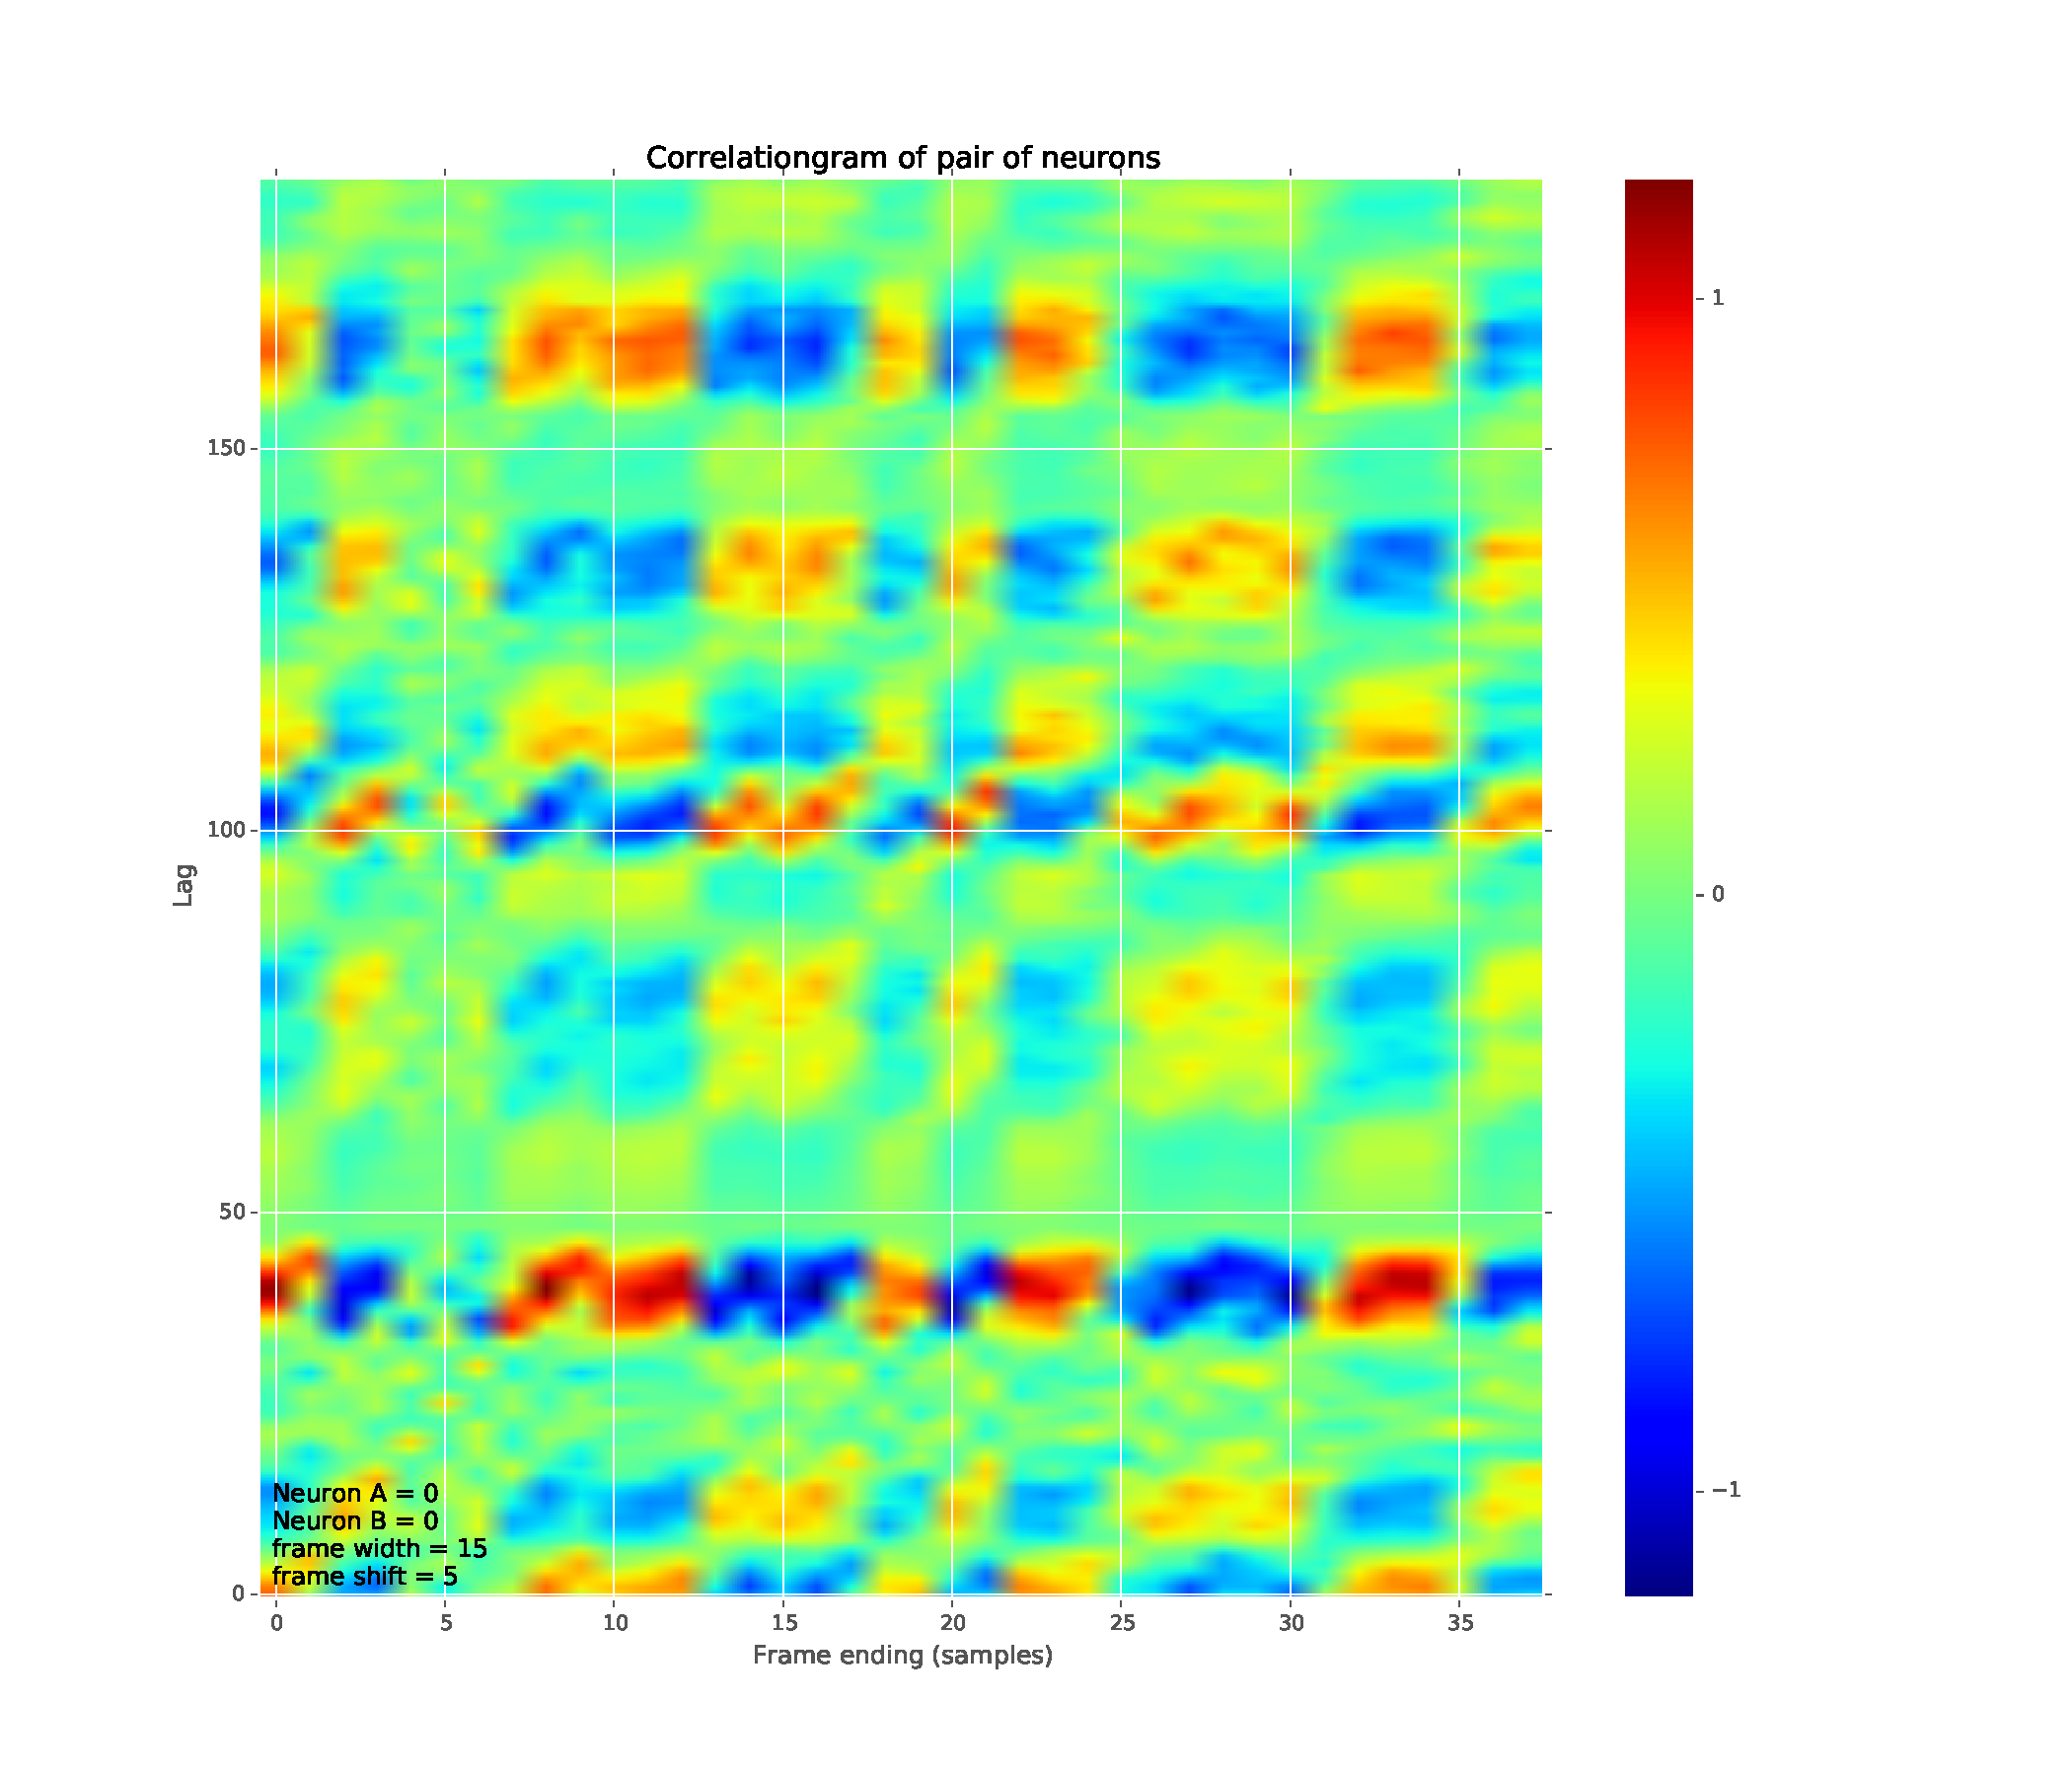
\includegraphics[width=\linewidth]{\plt/acfMain_corrGram_2016_02_05_16_49_00.pdf}
    \caption{Frame width = 15}
    \label{fig:ori_simple}
  \end{subfigure}%
  \begin{subfigure}[b]{0.5\textwidth}
    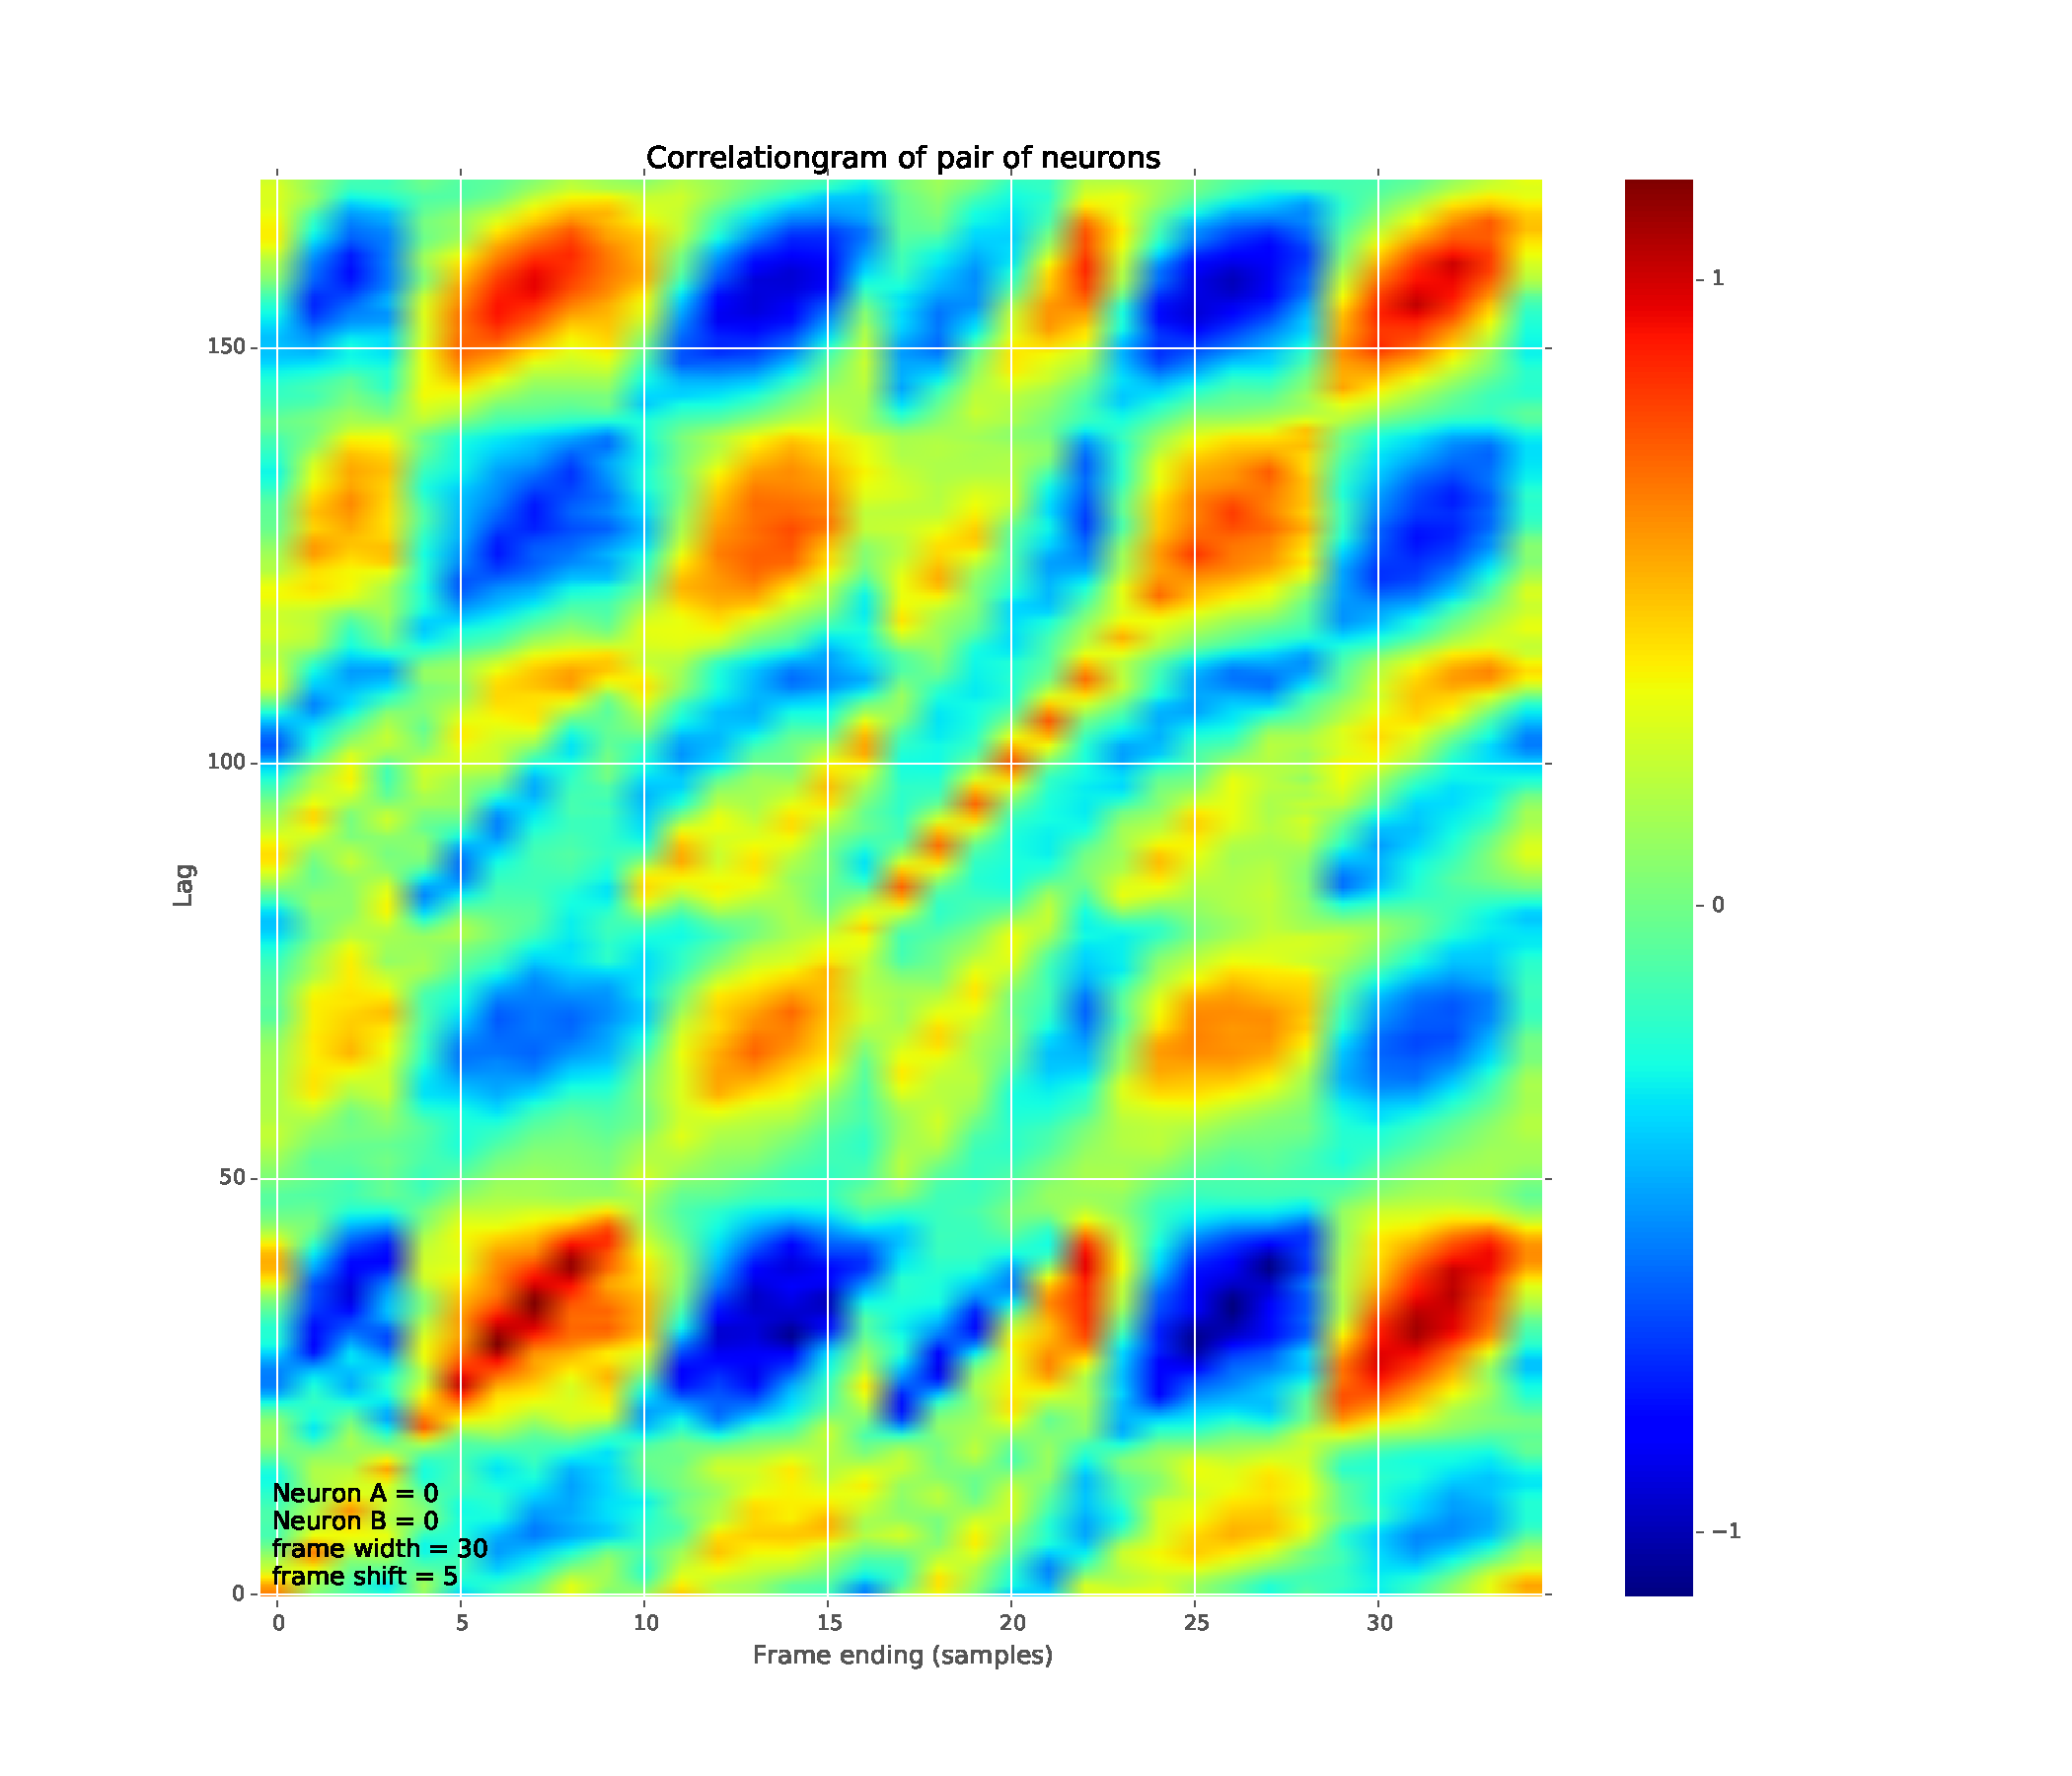
\includegraphics[width=\linewidth]{\plt/acfMain_corrGram_2016_02_05_16_49_10.pdf}
    \caption{Frame width = 30}
    \label{fig:acfgram_same}
  \end{subfigure}%
  \caption{ACFGram plots for template and target responses from same neuron.}\label{fig:oridir_simple}
\end{figure}
The Figure~\ref{fig:acfgram_diff} shows ACFGram plots for two different neuron responses. Motifs across neurons are studied for finding a better correlation metric. For different frame widths, responses indicate presence of motifs across neurons. The approximate length of motifs is more than 2 seconds, which is significant. Importantly, more or less any pair of neurons taken from the sampled set of 65 neurons from each mouse exhibited the presence of motifs. This indicates the inter neuronal correlation. This supports the claim that information in V1 is coded in population by inter-neuronal correlations.
\begin{figure}[h]
  \begin{subfigure}[b]{0.5\textwidth}
    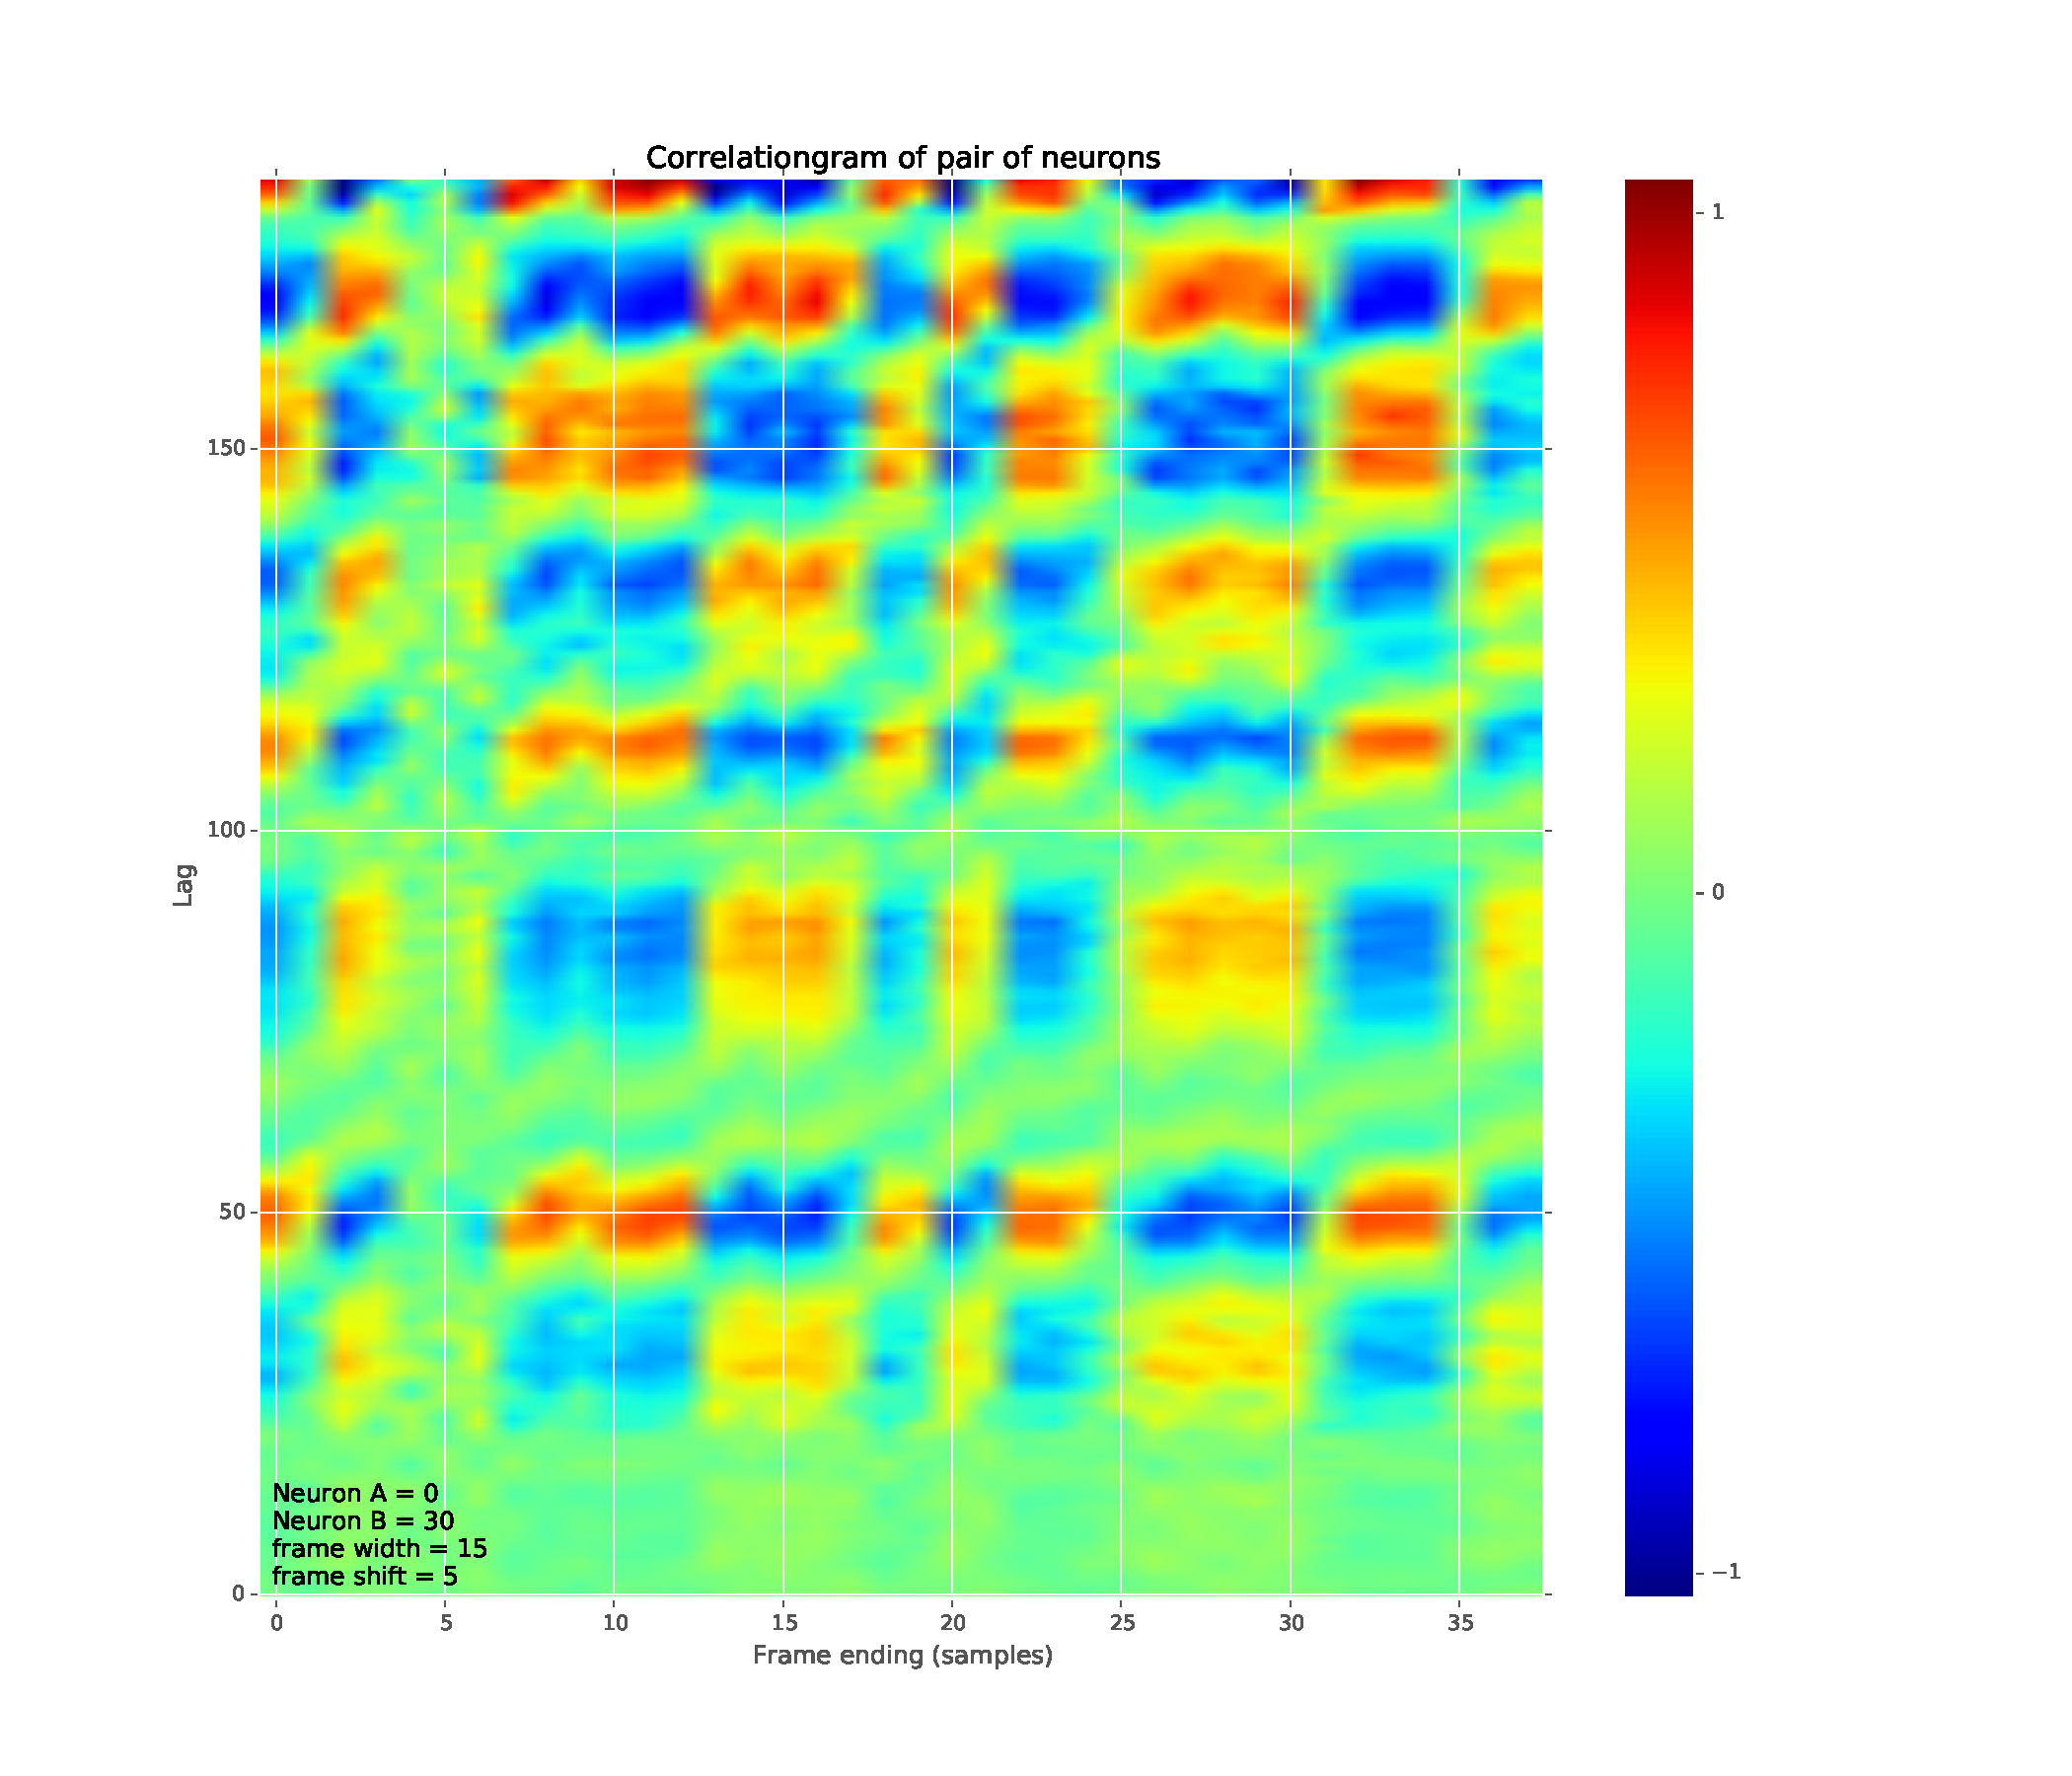
\includegraphics[width=\linewidth]{\plt/acfMain_corrGram_2016_02_05_16_45_22.pdf}
    \caption{Frame width = 15, frame shift = 5}
    \label{fig:ori_simple}
  \end{subfigure}%
  \begin{subfigure}[b]{0.5\textwidth}
    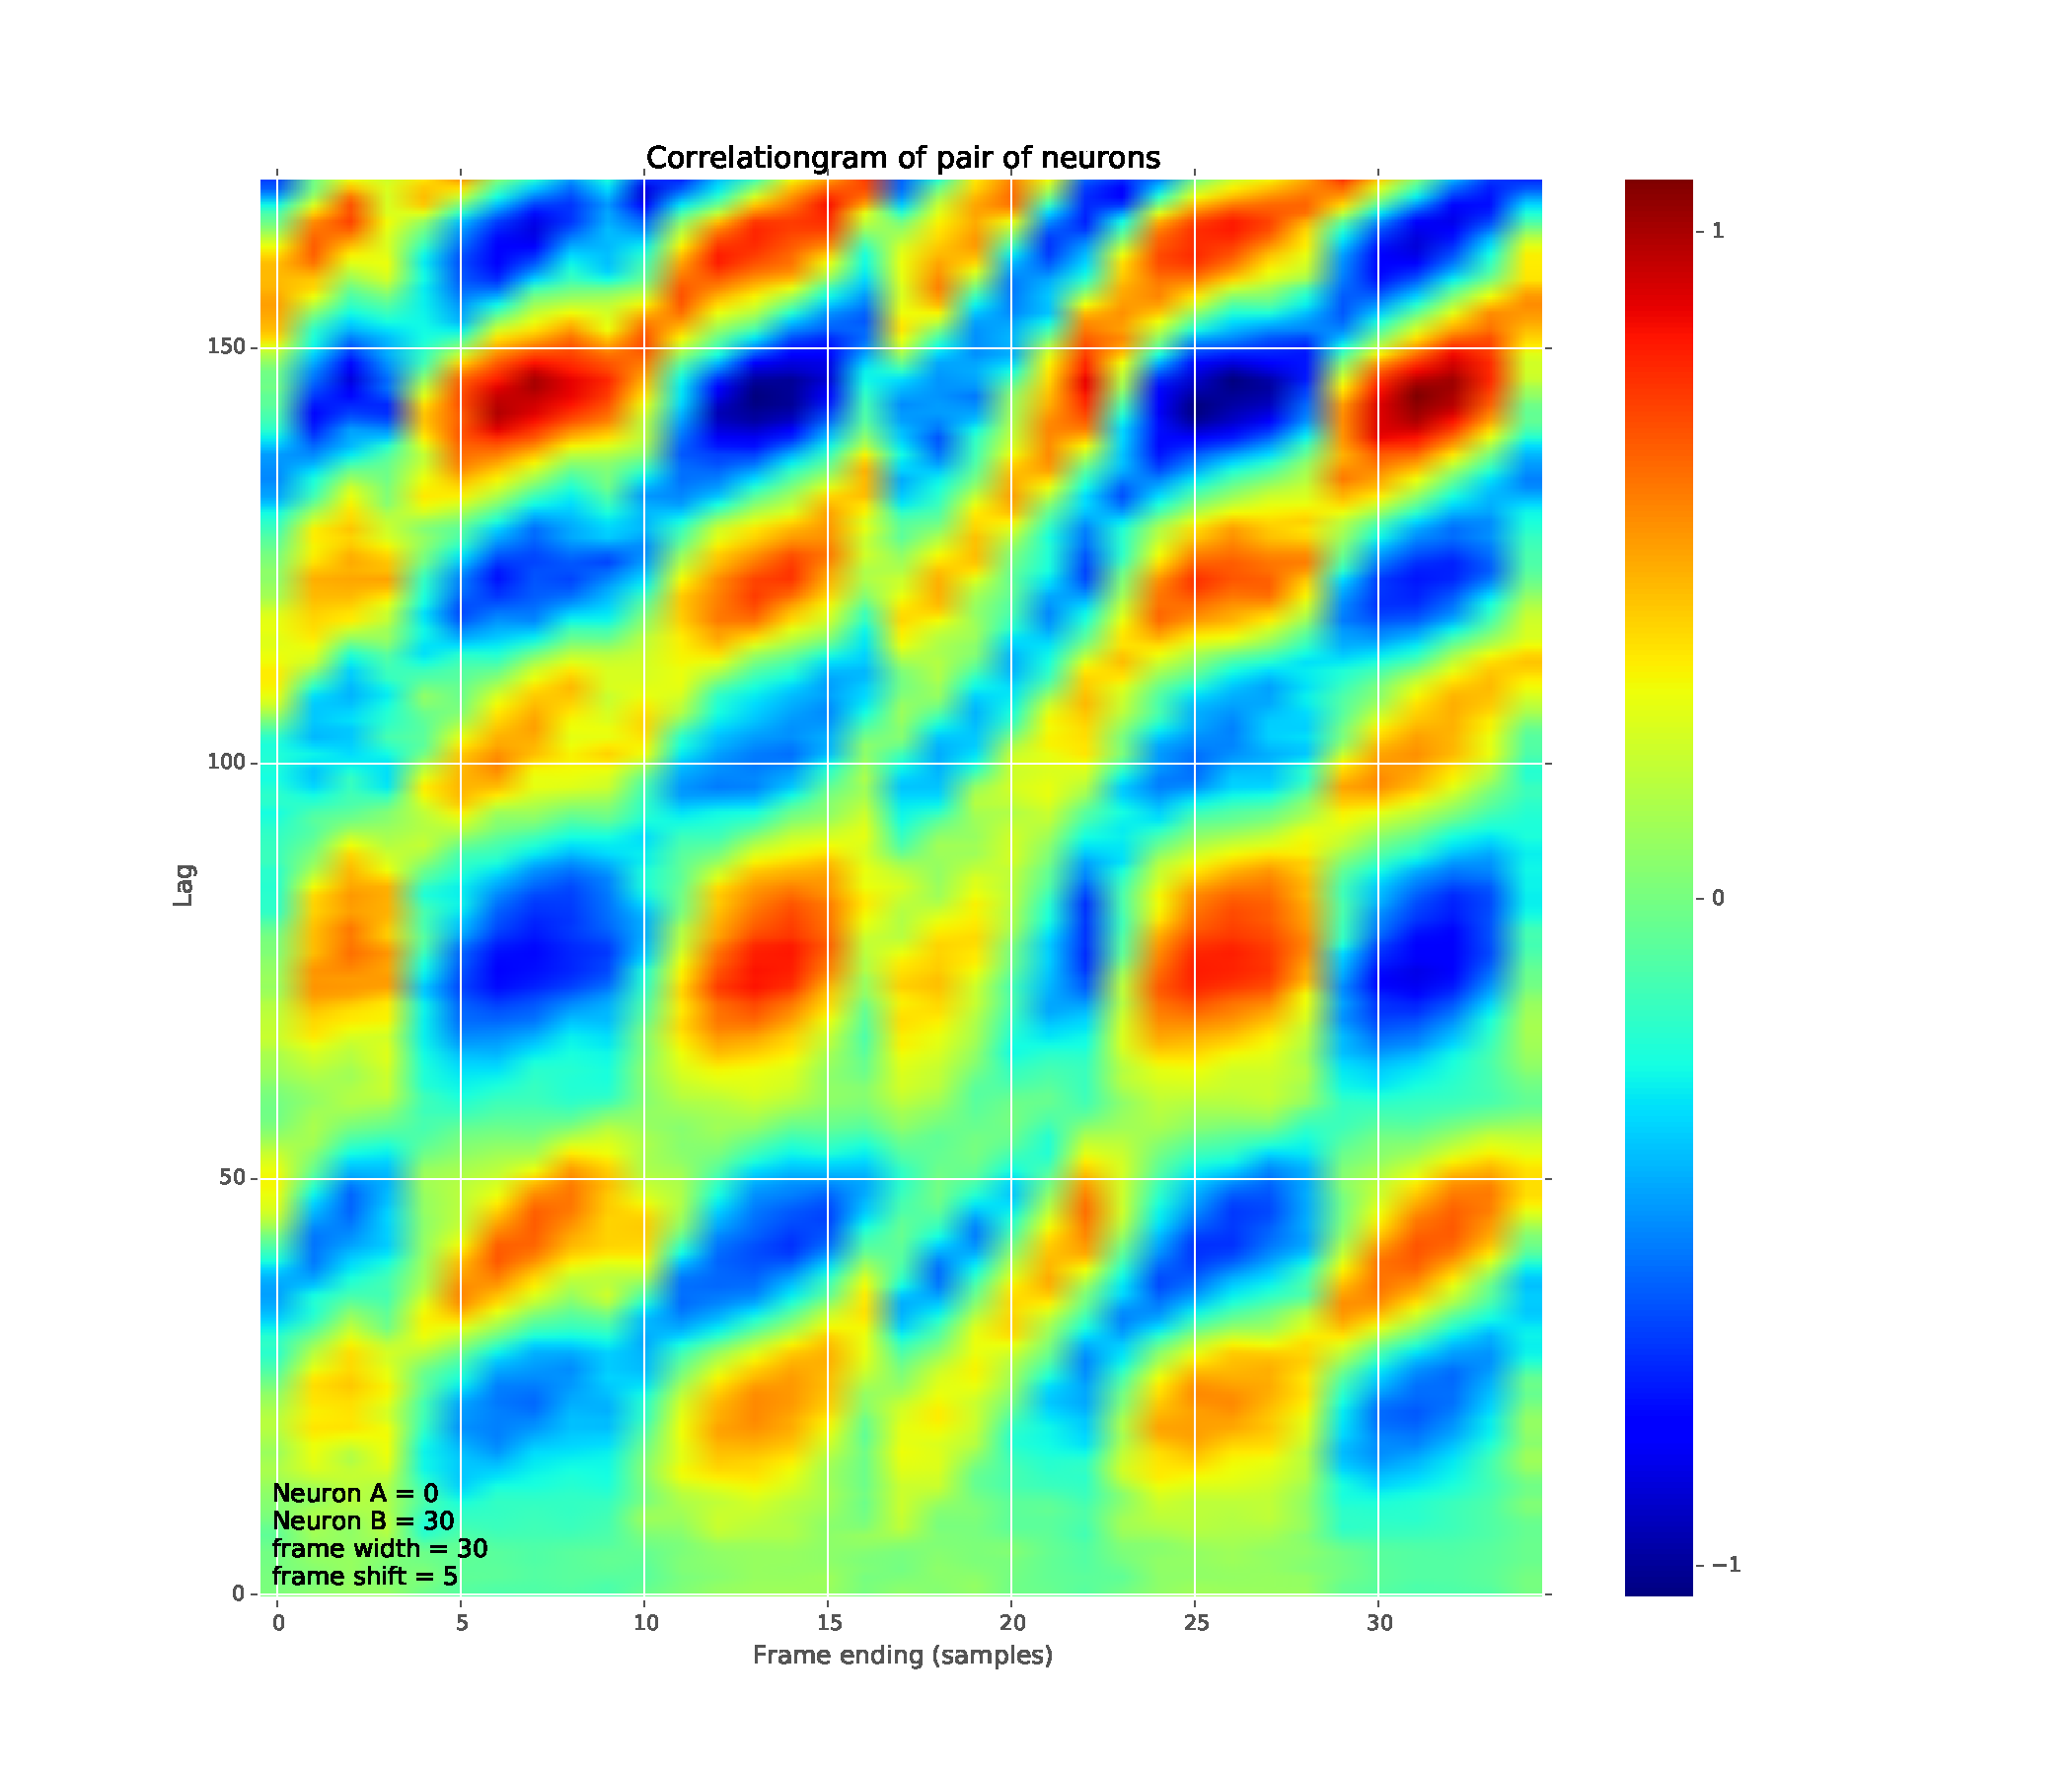
\includegraphics[width=\linewidth]{\plt/acfMain_corrGram_2016_02_05_16_45_38.pdf}
    \caption{Frame width = 30, frame shift = 5}
    \label{fig:acfgram_diff}
  \end{subfigure}%
  \caption{ACFGram plots for template and target responses from different neurons.}\label{fig:oridir_simple}
\end{figure}
The search for the presence of motifs in primary visual cortex succeeded in with experimentally verifying rough common subsequences of significance ($>2$ seconds) exists in neuronal responses. This motivates us to find the longest motifs you can find between two neurons. Also till now we used Pearson correlation as a measure of similarity. We look into rough measures of similarity and longest common subsequence in the next chapter.

% section acfgram (end)

%%%%%%%%%%%%%%%%%%%%%%%%%%%%%%%%%%%%%%%%%%%%%%%%%%%%%%%%%%%%%%%%%%%%%%
\chapter{Rough Longest Common Subsequence (RLCS)}     % 12 pages
\label{chap:rlcs}
Having established existence of motifs in neuronal responses, A robust algorithm to extract best possible motifs from two signals is required. As a longer motif has more significance in the context, an algorithm which produce longest common subsequence is desirable. Longest Common Subsequence (LCS) is a classical problem in query string matching, data comparison and Bio-informatics. We will eventually look into an adapted LCS problem which can be used to match signals called Rough Longest Common Subsequence (RLCS).

\section{Longest Common Subsequence (LCS)} % (fold)
\label{sec:longest_common_subsequence_}
A subsequence of a string $S$ is a set of characters that appear from left to right in original string $S$ but not necessarily consecutive. There will be more than one subsequence for any string with length greater than unity. For two strings $S_1$ and $S_2$, the common entries in sets of substrings of each strings are called common subsequences of $S_1$ and $S_2$. Among the common subsequences, the subsequence with maximal length is called Longest Common Subsequence. 

Some examples of LCS are given in Table~\ref{table:lcs_ex}. Note that there can be more than one LCS for two strings.
\begin{table}[h]
\centering
\begin{tabular}{|c | c| c|}
\hline
String 1 - $S_1$ & String 2 - $S_2$ & LCS($S_1, S_2$) \\
\hline
ABCDGH & AEDFHR & ADH \\
AGGTAB & GXTXAYB & GTAB \\
AGCAT  & GAC     & AC, GC and GA \\
BACDB & BDCB & BCB \\
\hline 
\end{tabular}
\caption{Some examples of LCS in string comparison}
\label{table:lcs_ex}
\end{table}

LCS problem can be defined formally for two subsequences $X = (x1, x2...xm)$ and $Y = (y1, y2...yn)$ as 
$$
LCS\left(X_{i},Y_{j}\right) =
\begin{cases}
  \empty
& \mbox{ if }\ i = 0 \mbox{ or }  j = 0 \\
  \textrm{  } LCS\left(X_{i-1},Y_{j-1}\right) \frown x_{i}
& \mbox{ if } x_i = y_j \\
  \mbox{longest}\left(LCS\left(X_{i},Y_{j-1}\right),LCS\left(X_{i-1},Y_{j}\right)\right)
& \mbox{ if } x_i \ne y_j \\
\end{cases}
$$

Where $X_i = (x1, x2...xi)$ and $Y_j = (y1, y2...yj)$.

LCS problem has an optimal substructure- the problem can be broken down into subproblems of similar kind. As the problem also has overlapping subproblems, a Dynamic Programming approach is used to find the LCS. Running time of the dynamic programming approach is  $O(nm)$ where n and m are the lengths of strings.
% section longest_common_subsequence_ (end)

\section{RLCS} % (fold)
\label{sec:rlcs}
LCS problem can be adapted for signal matching. Instead of equality, a rough distance measure is used. If the distance between samples is less than a threshold, they are considered a match. It is not desirable just to optimize the length of subsequence in signals as the gaps between selected samples can cause false alarms. Dynamic Programming optimization has to be penalizing gaps and motivating matches. The rest of the problem and the solution remains similar to LCS problem and similar Dynamic Programming approach can solve the problem efficiently.

Modified LCS problem with rough comparison is stated below. The RLCS of two input sequnces $X = <x1, x2...xm>$ and $Y = <y1, y2...yn>$ is obtained by maximizing the score value $S$.
$$
S\left(X_{i},Y_{j}\right) =
\begin{cases}
  0
& \mbox{ if }\ i = 0 \mbox{ or }  j = 0 \\
  \textrm{  } S\left(X_{i-1},Y_{j-1}\right) \frown x_{i}
& \mbox{ if } dist(x_i , y_j) < \tau_{dist} \\
  \mbox{max}\left(S\left(X_{i},Y_{j-1}\right),S\left(X_{i-1},Y_{j}\right)\right)
& \mbox{ if } dist(x_i , y_j) > \tau_{dist} \\
\end{cases}
$$
Where $X_i = <x1, x2...xi>$ and $Y_j = <y1, y2...yj>$.

Various context uses different distance measures for comparing samples.  Manhattan distance (city block distance) of notes is used in context of music matching [\cite{lin2011music}]. In a work on verification of Raga in Carnatic music [\cite{duttaraga}], a domain specific similarity measure is used. RLCS on neuronal signals in this work uses normalized Euclidean distance for checking similarity.
$$dist(x_i, y_i) = (x_i - y_j)^2$$
Distances are normalized from 0 to 1 by performing: 
$$dist(x_i, y_i) = \frac{dist(x_i, y_i) - minDist}{maxDist - minDist}$$
Where $minDist$ is the minimum pairwise distance and $maxDist$ is the maximum pairwise distance.

Most important part of RLCS is the adapted score update rules. In the classical LCS problem, the gaps between the selected subsequence was not considered; Instead only the length of the subsequence was of consideration. But in signals, having a gap in between will give poor signal match. So it is important to penalize the gaps and reward matches.
The following score update rules penalizes gaps in subsequence and awards positive score for matches.
\begin{enumerate}
  \item Score update for a match. $dist(x_i, y_j) < \tau_{dist}$\\
  $$score(i, j) = score(i - 1, j - 1) + 1 - \frac{dist(x_i, y_j)}{\tau_{dist}}$$
  This case happens when a match is found. The score should be rewarded with a positive value.  The maximum awarded score is 1 for an exact sample match and minimum score given is 0 for when the distance equals threshold. The closer the samples, more the score.
  \item Score update for a mismatch. $dist(x_i, y_j) > \tau_{dist}$\\
  $$score(i, j) = score(i - 1, j - 1) - \delta$$
  We allowed any number of gaps in a string LCS problem. But in the case of signals, we cannot allow large gaps as it would produce false alarms. We penalize each mismatching samples with a constant score $\delta$.
\end{enumerate}
The problem is then recursively solved using  Dynamic Programming algorithm which will provide us with a 2-D score matrix. The Dynamic programming algorithm for input sequences $X = <x_0, x_1, ..., x_{m-1}>$ and $Y = <y_0, y_1, ..., y_{n-1}>$ is explained in 

\begin{algorithm}
\caption{Dynamic Programming algorithm for RLCS ***}\label{euclid}
\begin{algorithmic}[1]
  \Function{RLCS}{X, Y, $\tau_{dist}$, $\delta$}
  \State $m \gets \text{length of }\textit{X}$
  \State $n \gets \text{length of }\textit{Y}$
  \State $p \gets min(m, n)$
  \For {$i = 0$; $i < m$; $i++$}
    \For {$j = 0$; $j < n$; $j++$}
      \State $dist(i, j) \gets euclideanDistance(x_i, y_j)$
    \EndFor
  \EndFor
  \State $\text{minDist} \gets min(dist)$ \Comment{For normalization}
  \State $\text{maxDist} \gets min(dist)$ \Comment{For normalization}\\

  \State $\text{cost} \gets zeros(m+2, n+2)$ \Comment{For storing running score}
  \State $\text{score} \gets zeros(m+2, n+2)$ \Comment{For storing score}
  \State $\text{diag} \gets zeros(m+2, n+2)$ \Comment{For backtracking}
  \State $\text{partial} \gets zeros(m+2, n+2)$ \Comment{For storing partial scores.}\\

  \For {$i = 0$; $i < m$; $i++$}
    \For {$j = 0$; $j < n$; $j++$}
      \State $d \gets (dist(i, j) - \text{minDist})/(\text{maxDist} - \text{minDist})$ 
      \Comment{Normalize}
      \If {($d < \tau{dist}$)} 
        \State $\text{diag }(i, j) \gets ` \nearrow '$\Comment{Path to travel while backtracking}
        \State $\text{cost }(i, j) \gets \text{cost }(i-1, j-1) + (1 - d/\tau_{dist})$
        \State $\text{score }(i, j) = \text{score }(i-1, j-1)$
      \ElsIf {$\text{cost }(i-1, j) > \text{cost }(i, j-1)$}
        \State $\text{diag }(i, j) \gets ` \uparrow'$
        \State $\text{cost }(i, j) = \text{cost }(i-1, j) - \delta$\Comment{Penalize}

        
      \EndIf

    \EndFor
  \EndFor
  \If {$i > \textit{stringlen}$} \Return false
  \EndIf
  \State $j \gets \textit{patlen}$
  \BState \emph{loop}:
  \If {$\textit{string}(i) = \textit{path}(j)$}
  \State $j \gets j-1$.
  \State $i \gets i-1$.
  \State \textbf{goto} \emph{loop}.
  \State \textbf{close};
  \EndIf
  \State $i \gets i+\max(\textit{delta}_1(\textit{string}(i)),\textit{delta}_2(j))$.
  \State \textbf{goto} \emph{top}.
  \EndFunction
\end{algorithmic}
\end{algorithm}


Backtracking through score matrix will gives us the Longest Common Subsequence. As we have been penalizing gaps, there will be points in the track where score is zero. For each sample match we had increased score and decreased for gaps. So the zero will mean that there are enough mismatches to balance the positive score created by matches. This lets us identify the boundary of a subsequence. A number of subsequences could be extracted by cutting at points where score goes zero. This set of subsequences are called \textbf{Longest Common Subsequence Set} (LCSS) [\cite{duttaraga}]. Algorithm ** explains backtracking to extract the LCSS.

\begin{algorithm}
\caption{Dynamic Programming algorithm for RLCS ***}\label{euclid}
\begin{algorithmic}[1]
  \Function{RLCS}{X, Y, $\tau_{dist}$, $\delta$}
  \State $m \gets \text{length of }\textit{X}$
  \State $n \gets \text{length of }\textit{Y}$
  \State $p \gets min(m, n)$
  \For {$i = 0$; $i < m$; $i++$}
    \For {$j = 0$; $j < n$; $j++$}
      \State $dist(i, j) \gets euclideanDistance(x_i, y_j)$
    \EndFor
  \EndFor
  \State $\text{minDist} \gets min(dist)$ \Comment{For normalization}
  \State $\text{maxDist} \gets min(dist)$ \Comment{For normalization}\\

  \State $\text{cost} \gets zeros(m+2, n+2)$ \Comment{For storing running score}
  \State $\text{score} \gets zeros(m+2, n+2)$ \Comment{For storing score}
  \State $\text{diag} \gets zeros(m+2, n+2)$ \Comment{For backtracking}
  \State $\text{partial} \gets zeros(m+2, n+2)$ \Comment{For storing partial scores.}\\

  \For {$i = 0$; $i < m$; $i++$}
    \For {$j = 0$; $j < n$; $j++$}
      \State $d \gets (dist(i, j) - \text{minDist})/(\text{maxDist} - \text{minDist})$ 
      \Comment{Normalize}
    \EndFor
  \EndFor
  \EndFunction
\end{algorithmic}
\end{algorithm}
\subsection{Motivic analysis of Neuronal signals with RLCS} % (fold)
\label{sub:motivic_analysis_of_neuronal_signals_with_rlcs}
Having established presence of motifs in neuronal responses, we use Rough Longest Common Subsequence (RLCS) algorithm to find the `best' motifs from a signal processing point of view. Penalizing the gaps makes RLCS a good signal matching algorithm.

The experiment was conducted on responses of neurons from V1 of 11 mice to different visual stimuli. Each signal is sampled at 20 Hz and last for 10 seconds. The study is split into different sections based on which neurons the signals come from.
\subsubsection{Motifs in responses of a neuron to different trials} % (fold)
\label{ssub:motifs_in_responses_of_a_neuron_to_different_trials}
The signals from a neuron's response to different trials of same stimuli are passed to RLCS algorithm to detect motifs. The score matrix in Figure 
% subsubsection motifs_in_responses_of_a_neuron_to_different_trials (end)
\subsubsection{Motifs in responses of two neurons in a mice} % (fold)
\label{ssub:motifs_in_responses_of_two_neurons_in_a_mice}

% subsubsection motifs_in_responses_of_two_neurons_in_a_mice (end)
\subsubsection{Motifs in responses of neurons across different mice} % (fold)
\label{ssub:motifs_in_responses_of_neurons_across_different_mice}

% subsubsection motifs_in_responses_of_neurons_across_different_mice (end)
% subsection motivic_analysis_of_neuronal_signals_with_rlcs (end)
\subsection{Normalized RLCS score as a correlation metric} % (fold)
\label{sub:normalized_rlcs_score_as_a_correlation_metric}

% subsection normalized_rlcs_score_as_a_correlation_metric (end)
% section rlcs (end)

%%%%%%%%%%%%%%%%%%%%%%%%%%%%%%%%%%%%%%%%%%%%%%%%%%%%%%%%%%%%%%%%%%%%%%
\chapter{Inferences and Future work}    % 3 pages
\label{chap:summary}

%%%%%%%%%%%%%%%%%%%%%%%%%%%%%%%%%%%%%%%%%%%%%%%%%%%%%%%%%%%%%%%%%%%%%%
\appendix
\chapter{Neural visual pathway}

%%%%%%%%%%%%%%%%%%%%%%%%%%%%%%%%%%%%%%%%%%%%%%%%%%%%%%%%%%%%%%%%%%%%%%
% Bibliography.
\pagebreak
\begin{singlespace}
  \begin{small}
	\bibliography{refs}
  \end{small}
\end{singlespace}
%%%%%%%%%%%%%%%%%%%%%%%%%%%%%%%%%%%%%%%%%%%%%%%%%%%%%%%%%%%%%%%%%%%%%%
\end{document}
